\chapter{Fortschreitende Elektronikentwicklung}\label{cha:Elektronikentwicklung}

In diesem Kapitel der Arbeit wird die Umsetzung der diversen Konzept und Strukturanforderungen in Hardware betrachtet. Dabei werden hier ausgesuchte Beispiele aus mehreren Vergangenen Jahren Vorgestellt und Technisch erläutert.
Dabei wird die kontinuierlich Fortschreitende Implementierung von Erfahrung im Zusammenspiel mit dem Modularen Gesamtkonzept aufgezeigt.

\section{Ursprünglicher Elektronikzustand}

Die in der Saison 2014 begonnen Voruntersuchungen fanden mit dem Flugsystem 'Maya' statt.
Abseits von Strukturellen und Flugmechanischen Problemen war auch die Elektronik eine kontinuierliche Quelle von Fehlern und Ausfällen des Flugzeugs.
Dies war größtenteils auf die Mangelnde Erfahrung im Umgang mit einem System eines solchen Komplexitätgrades zurückzuführen.Aber auch eine noch unzureichende Ausstattung mit Werkzeug,  Testmöglichkeiten und Methoden in Kombination mit der Unübersichtlichen Kabelführung erschwerte die Fehlersuche.
Auch die ersten versuche mit einem selbst gebauten Flächenmodell waren mit ähnlichen Schwierigkeiten in der Elektronik behaftet.

\begin{figure}[H]
\centering
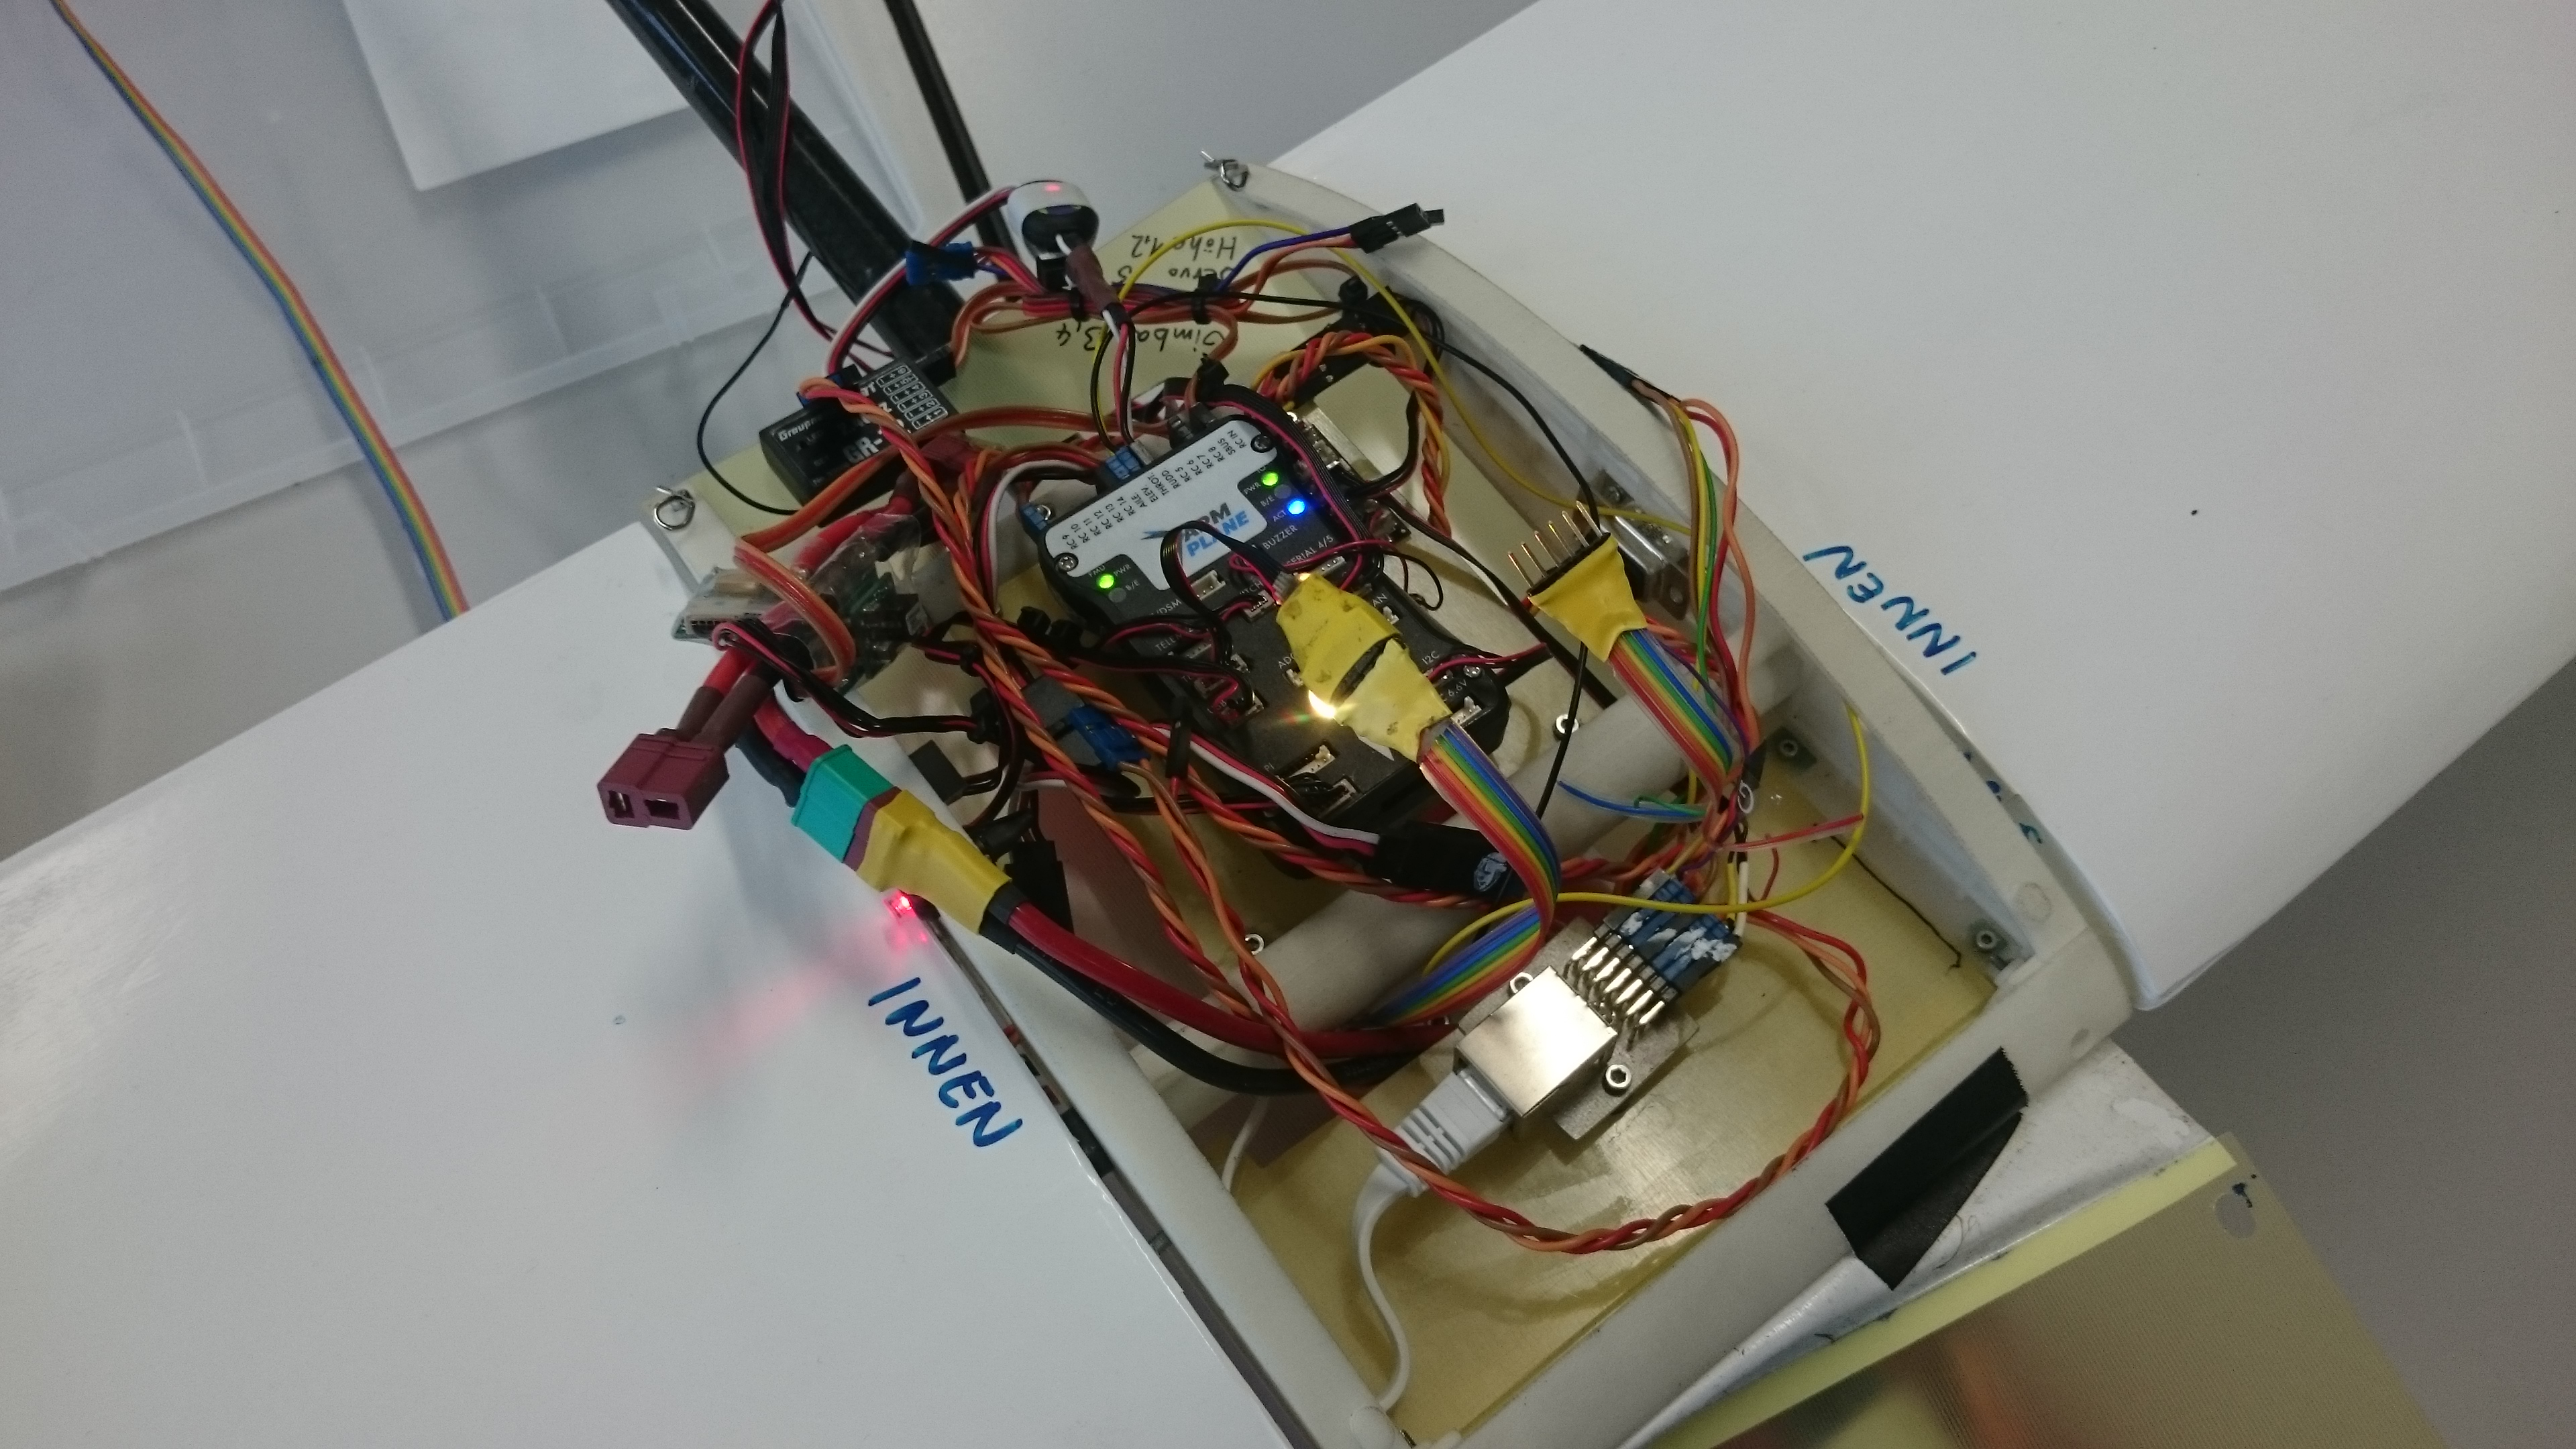
\includegraphics[width=0.9\textwidth]{bilder/Fotos/Elektronik_Kabelsalat_2015.jpg} 
\caption{Anblick der Elektronik zu Beginn 2015} 
\label{Anblick der Elektronik zu Beginn 2015}
\end{figure}

\section{Neue Platinenaufteilung}

Aus diesen Erfahrungen entstand das Eingangs vorgestellte Konzept für die Elektronik des Fliegers.
Dieses Konzept wurde 2015 erstmals angewandt, um eine Übersichtliche und einfach handhabbare Hardwareplattform mit leicht überprüfbaren Funktionen Umzusetzen.

\subsection{Leistungsplatine}

\subsubsection{Schaltplan}

\begin{figure}[H]
\centering
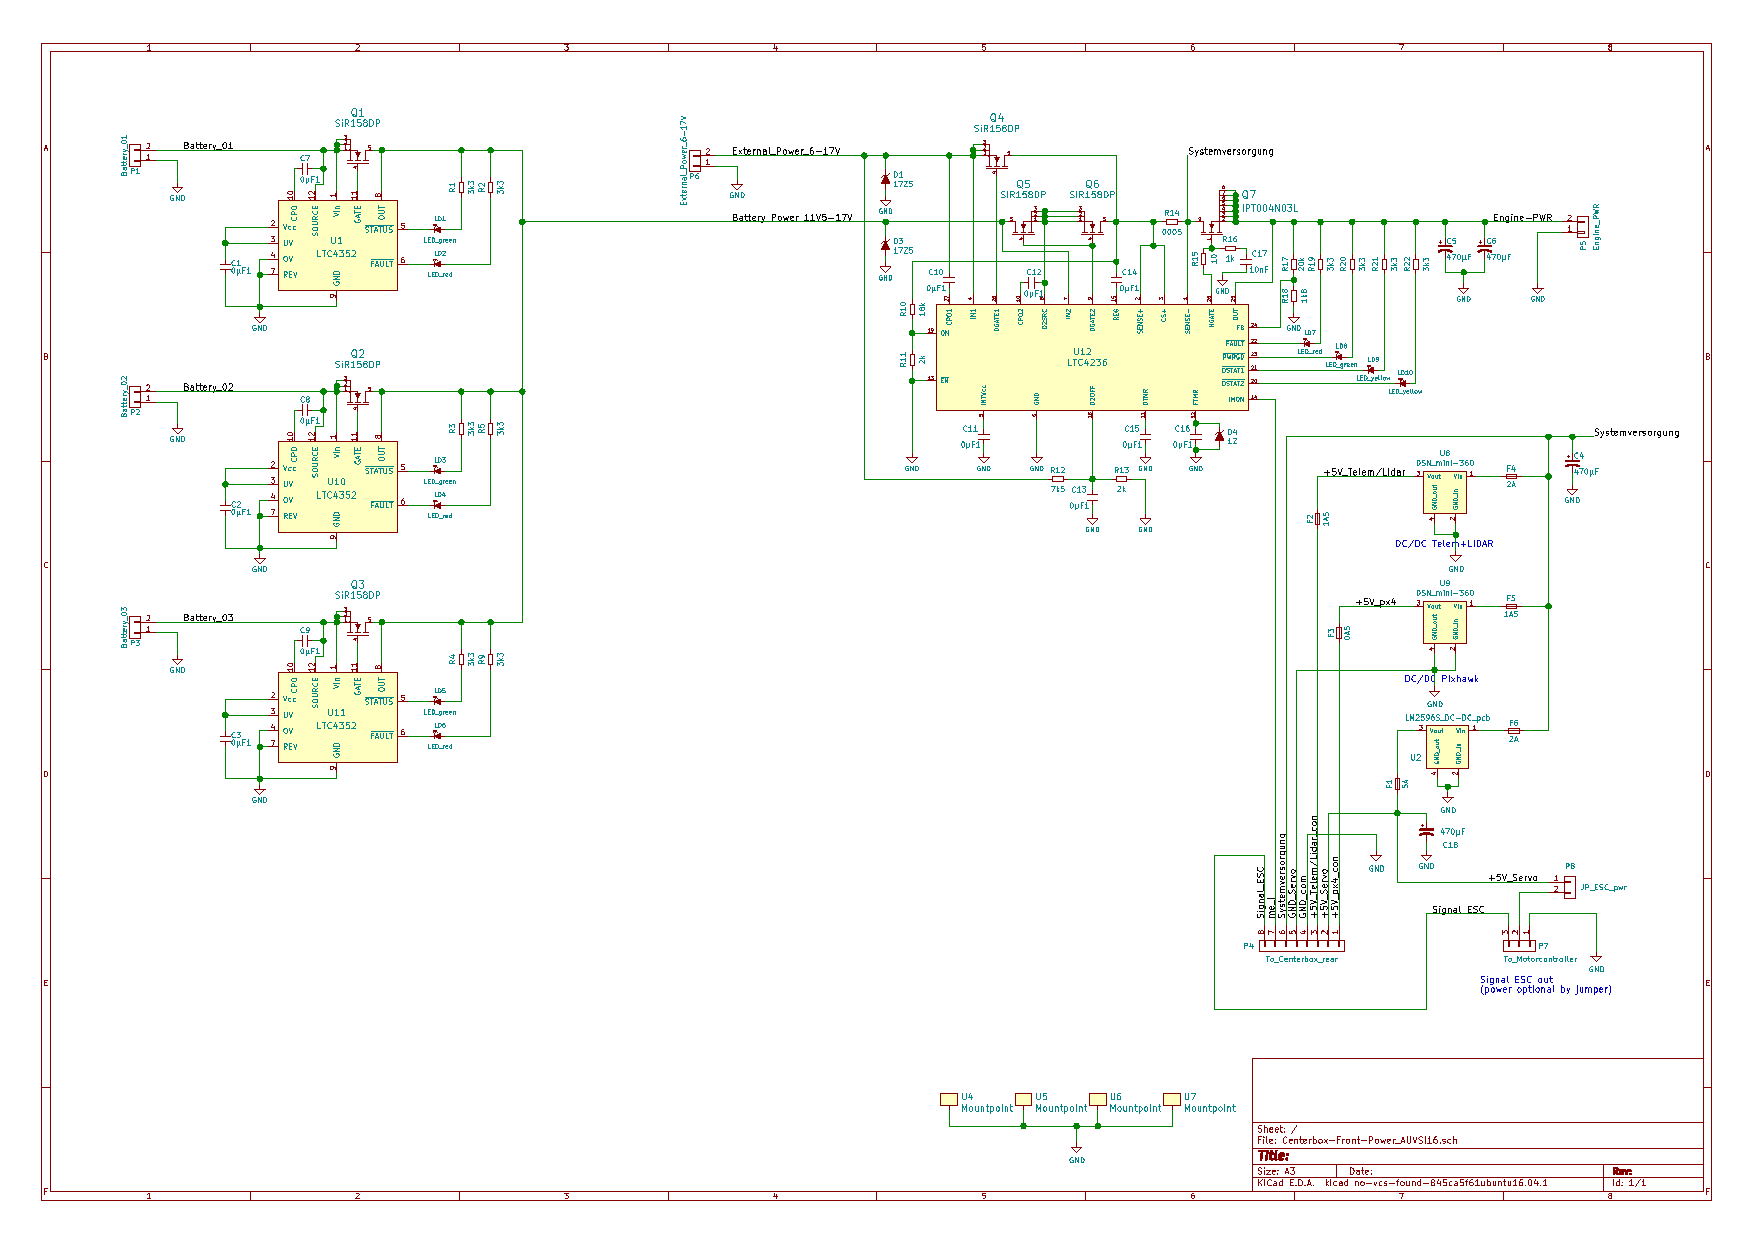
\includegraphics[width=0.9\textwidth]{bilder/Centerbox/Centerbox-Front-Power_AUVSI16.pdf} 
\caption{Schaltplan der Leistungsplatine} 
\label{fig:Schaltplan der Leistungsplatine}
\end{figure}

\subsubsection{Platinenlayout}

\begin{figure}[H]
\centering
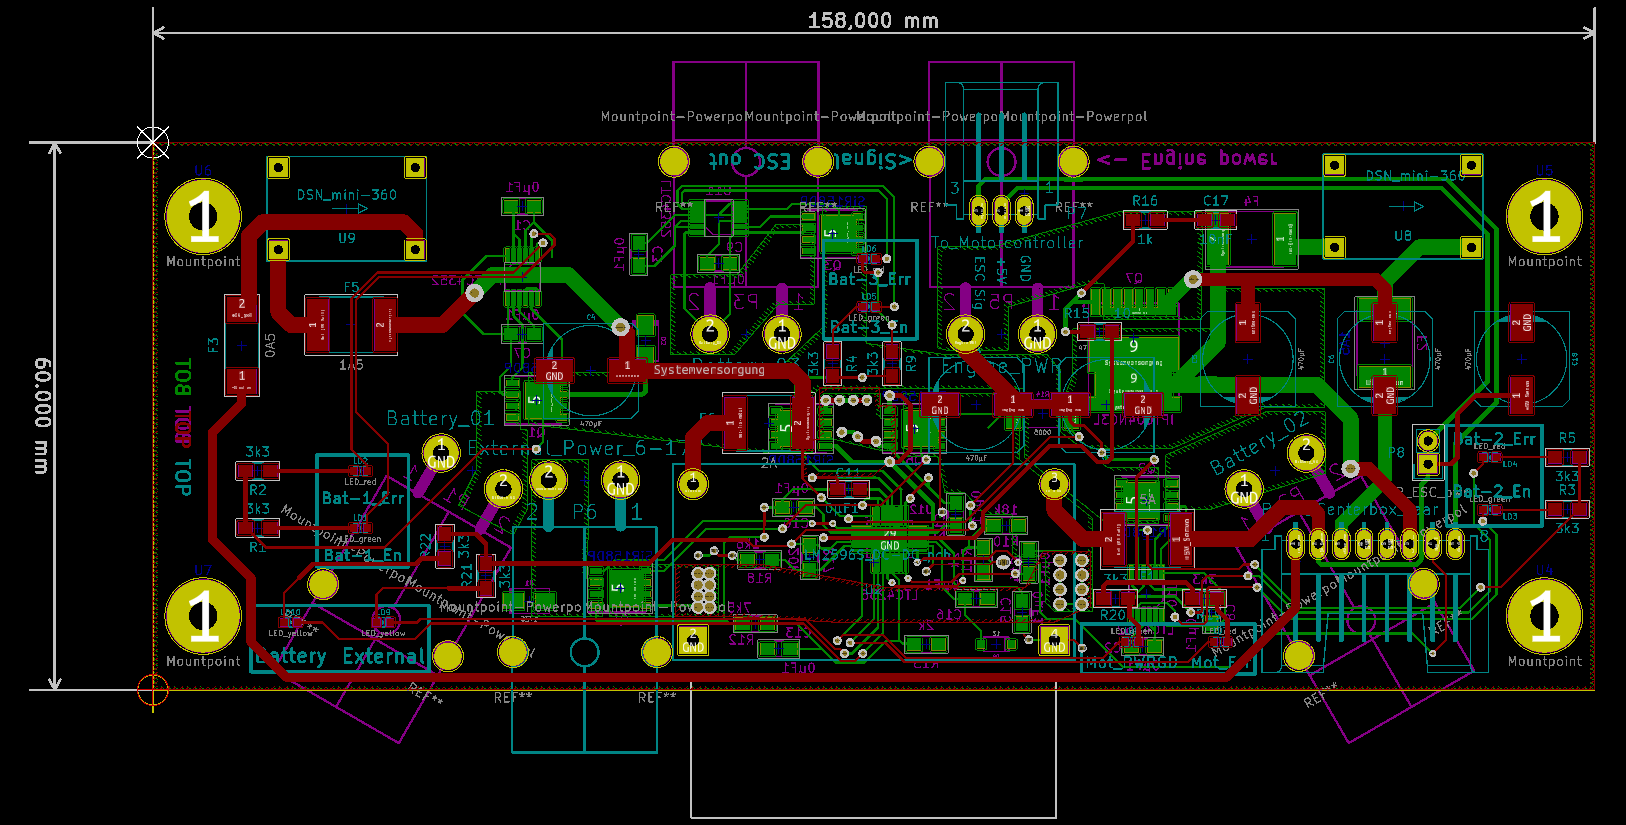
\includegraphics[width=0.9\textwidth]{bilder/Centerbox/Centerbox-Front-Power_AUVSI_2016_rev-01_layout.png} 
\caption{Layout der Leistungsplatine} 
\label{fig:Layout der Leistungsplatine}
\end{figure}


\subsection{Autopilotenplatine}

\subsubsection{Schaltplan}

\begin{figure}[H]
\centering
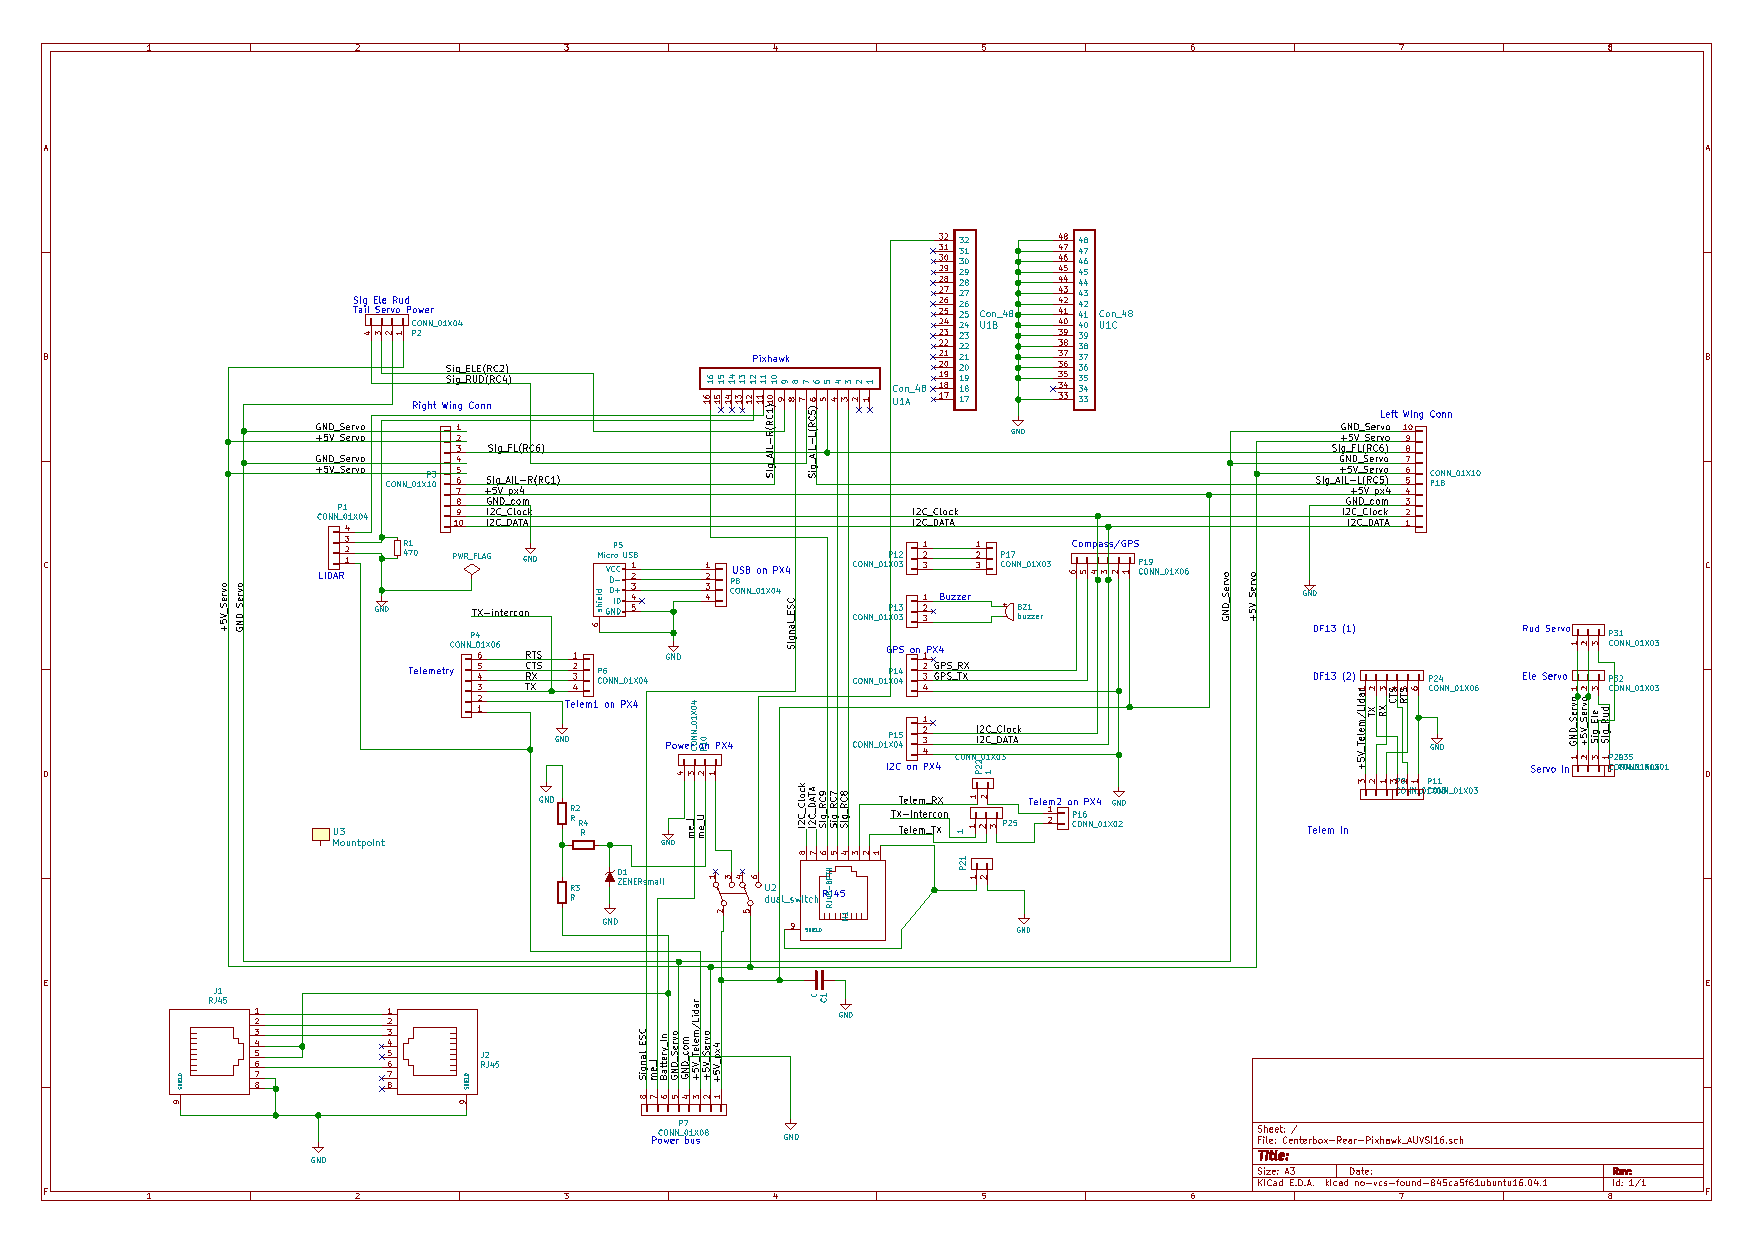
\includegraphics[width=0.9\textwidth]{bilder/Centerbox/Centerbox-Rear-Pixhawk_AUVSI16.pdf} 
\caption{Schaltplan der Autopilotenplatine} 
\label{fig:Schaltplan der Autopilotenplatine}
\end{figure}

\subsubsection{Platinenlayout}

\begin{figure}[H]
\centering
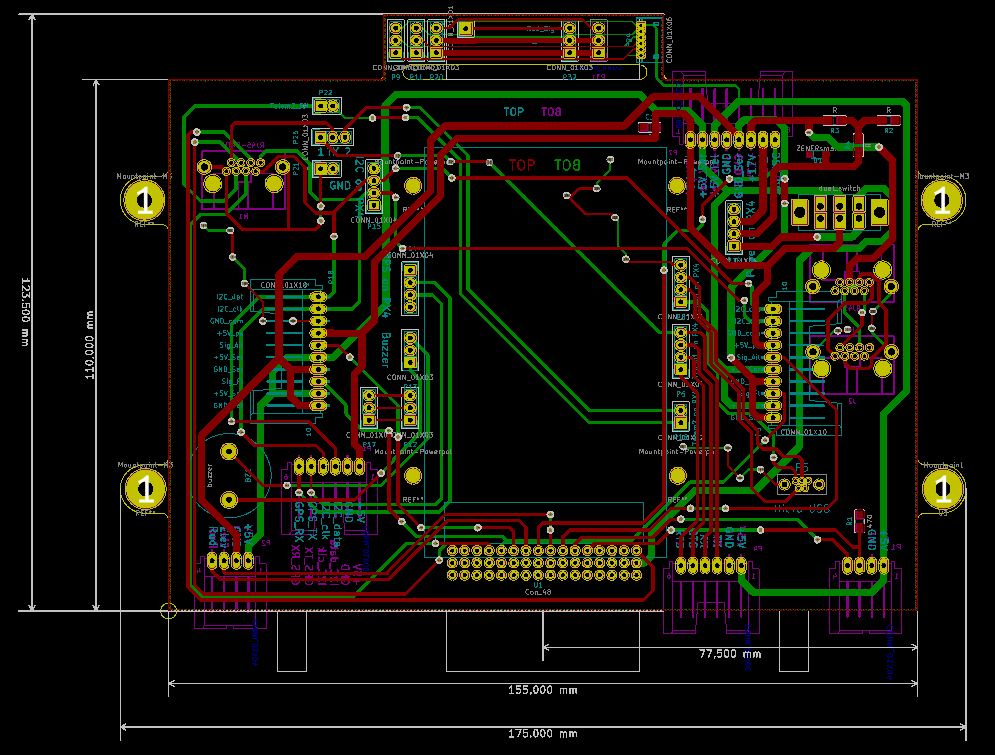
\includegraphics[width=0.9\textwidth]{bilder/Centerbox/Centerbox-Rear-Pixhawk_AUVSI_2016_rev-01-layout.png} 
\caption{Layout der Autopilotenplatine} 
\label{fig:Layout der Autopilotenplatine}
\end{figure}

\section{Bedien- und Schutz Konzepte}

\subsection{Eineindeutige Verbinderauswahl}

Für die angepasste Führung von Leistungspfaden und Signalpfaden wurden im Laufe des bisherigen Projekts je zwei verschiedene Steckersysteme eingesetzt.
Die Leistungsverbinder sind lediglich in Plus und Minuspol aufgeteilt und die Korrekte Montage wird über eine Mechanische Kodierung sichergestellt.
Bei den Signalverbindern wird eine mechanische Kodierung über eine einmalige Anzahl an Kontakten angestrebt.So kann in Verbindung mit der konsequenten Beschriftung aller Gegenstellen auf der Platinenseite eine fehlerhafte Montage quasi ausgeschlossen werden. Dabei werden zum teil auch bewusst Steckverbinder mit mehr Kontakten als zu übertragenden signalen ausgewählt um diese Einendeutikeit zu erreichen.

Die Hochstromverbindungen werden stets mit Kabelquerschnitten von 1,5 mm ausgeführt. Der Mantel besteht aus PVC außer in der Nähe von heißen Bauteilen an denen Silikon zum einsatz kommt.
Zu beginn wurden als Hochstromstecker Bauteile des Typs XT60 der Firma hexTronik verwendet.
Diese werden von den meisten Zukaufbaugruppen der Pixhawk Systems verwendet und ermöglichten eine mechanisch kodierte eindeutige Verbindung.
Sie sind für Ströme von 60 Ampere und Spannungen von 120 V freigegeben.
Jeoch waren diese Steckverbinder nur zur Lötmontage vorgesehen. Es wurde die Erfahrung gemacht das die Verbindungen zur Kabelseite immer wieder versagten. Teils wegen Qualitativ ungenügender Lötstellen, teils wegen Brüchen durch Handhabung mit Bewegung des Kabels am Übergang von der Lötstelle zum Kupferkabel am Steifigkeitssprung.

-->> Bild von XT60 und Powepol 55 

Daraufhin wurde ein neues System mit Crimpmontage gesucht.
Hierfür wurde das System POWERPOLE 45 der Firma Anderson Power Products ausgewählt. Die Steckverbinder sind bis zu einem Dauerstrom von 55 Ampere und einer Spannung von 300 V freigegeben.
Die Kabelbrüche wurden mit dem Ersatz der Lötverbidungen durch das Crimpsystem beseitigt. Sie können in den Quadratischen Gehäusen beliebig nebeneinander eingeclipt werden was größere Steckblöcke ermöglicht. Jedoch führte diese variable Montierbarkeit auch immer wieder zu wiedersprüchlicher Montage von Ladekabeln und Akkus bezüglich der Polposition.
Außer einer klaren Standardisierung der Polung wurde bisher noch keine Konzept gefunden Bedienfehler auszuschließen. 

Beide Systeme verwenden das Prinzip des Kraftschlusses für die Fixierung der Steckverbindung. Die für Montage und Demontage nötigen Kräfte sind jedoch an beengten Stellen im Flieger immer wieder hinderlich bei der Handhabung. Deshalb wird eine Formschlussbasierte Fixierung ähnlich den Signal Steckverbindern erwogen.


Für die Verbindung von Signalleitungen  und Versorgungsleitungen mit kleinen Strömen wurde zu Beginn das Stecksystem MSF der Firma Lumberg verwendet.
Dieses ist für 5 A je Pin bei bis zu 160 V freigegeben. Die Fixierung der Verbindung erfolgt hier über Formschluss in Form einer Lasche im Platinensockel des Verbinders welcher eine Nase am Stecker blockiert. Darüber hinaus besteht noch eine gewisser Kraftschluss über die Kontakte der bei der Demontage der Verbindung oft als unerwünscht hoch eingestuft wurde.


Als Alternative wurden die Verbinder aus der PA Reihe der Firma JST erprobt und mittlerweile in den Einsatz überführt.
Die Stecker sind für 3 A je Pin bei maximal 250 V freigegeben.
Die Fixierung wird auch hier über Formschluss in Gestalt einer Hakennase am Kabelseitigen Stecker realisiert.
Die Verbinder haben sich bisher bewährt, da sie einen guten Kompromiss aus kompakterer Baugröße und guter Handhabung in Montage und Demontage gegenüber den bisher verwendeten MSF Verbindern darstellen.
Die Reduzierte Strombelastbarkeit stellt in der Praxis keinen Nachteil dar.Die Logiksignale bringen nur Ströme im mA Bereich auf und auch die Servoversorgung leitet maximal 1 A.

\begin{figure}[H]

\begin{subfigure}{}
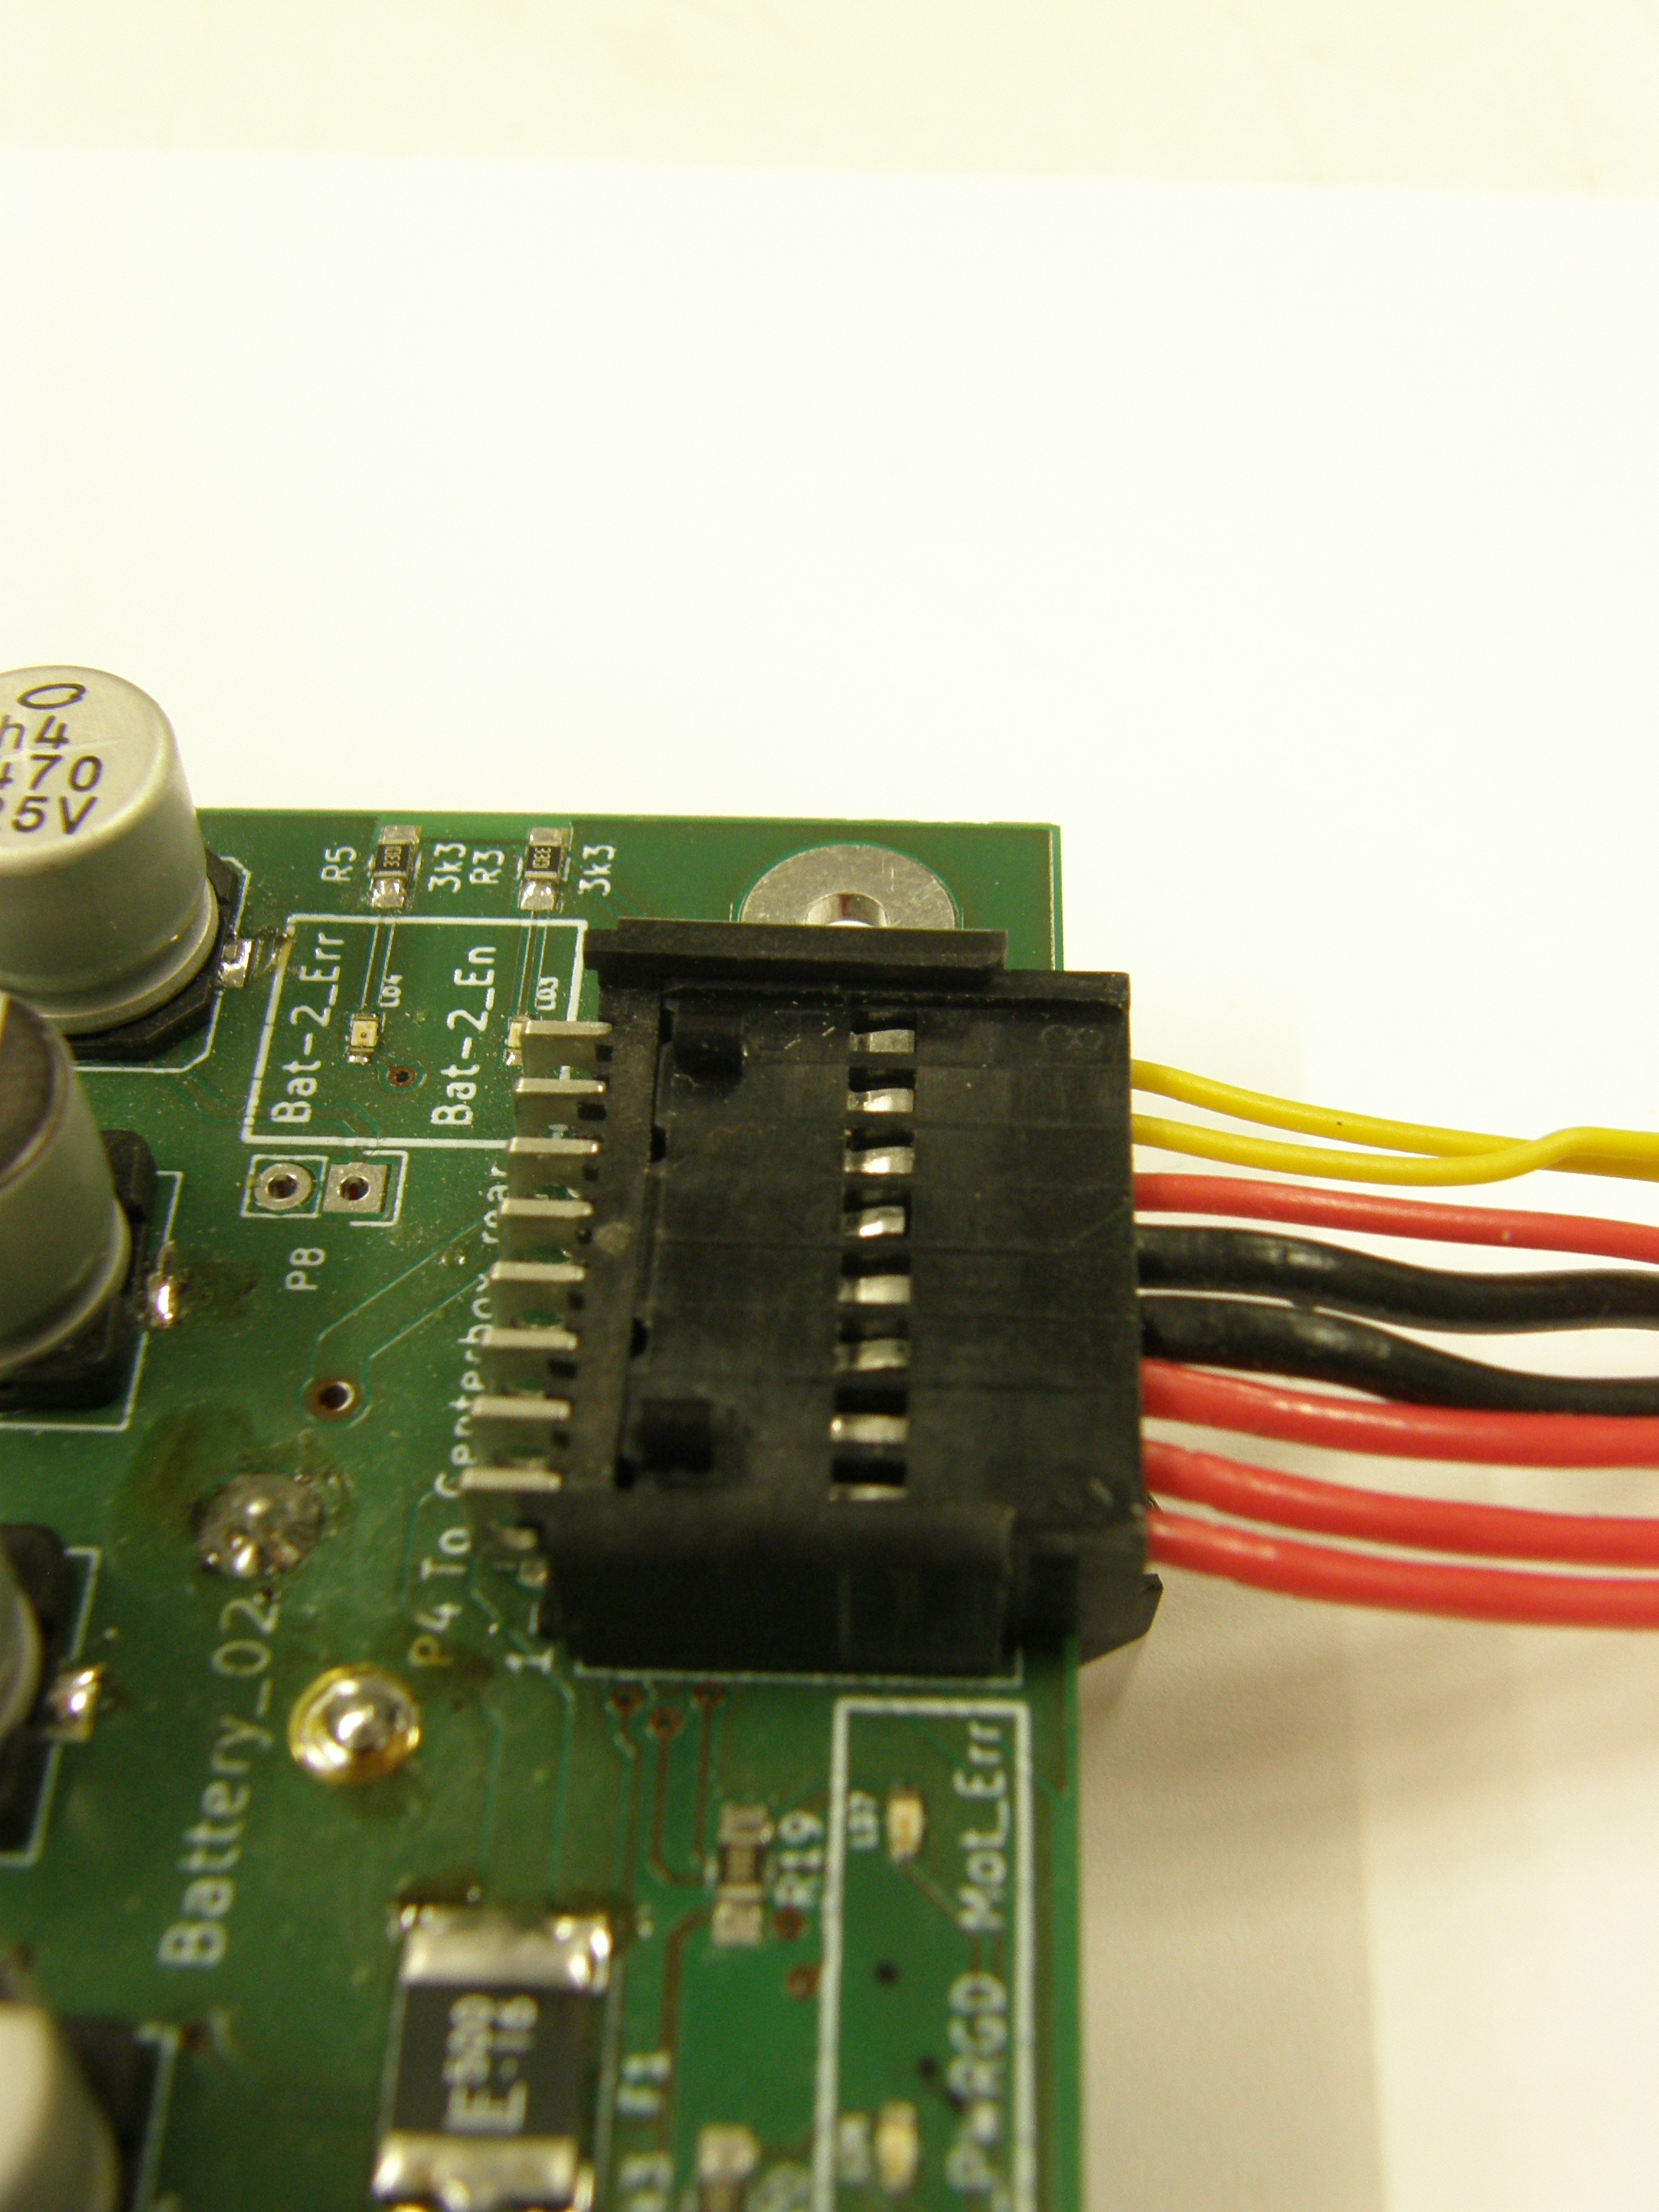
\includegraphics[width=0.6\textwidth, center]{bilder/Stecker/Stecker_Lumberg_MSF.jpg} 
\caption{Der ursprünglich eingesetzte Lumberg MSF Steckverbinder} 
\label{fig:Der ursprünglich eingesetzte Lumberg MSF Steckverbinder}
\end{subfigure}

\begin{subfigure}{}
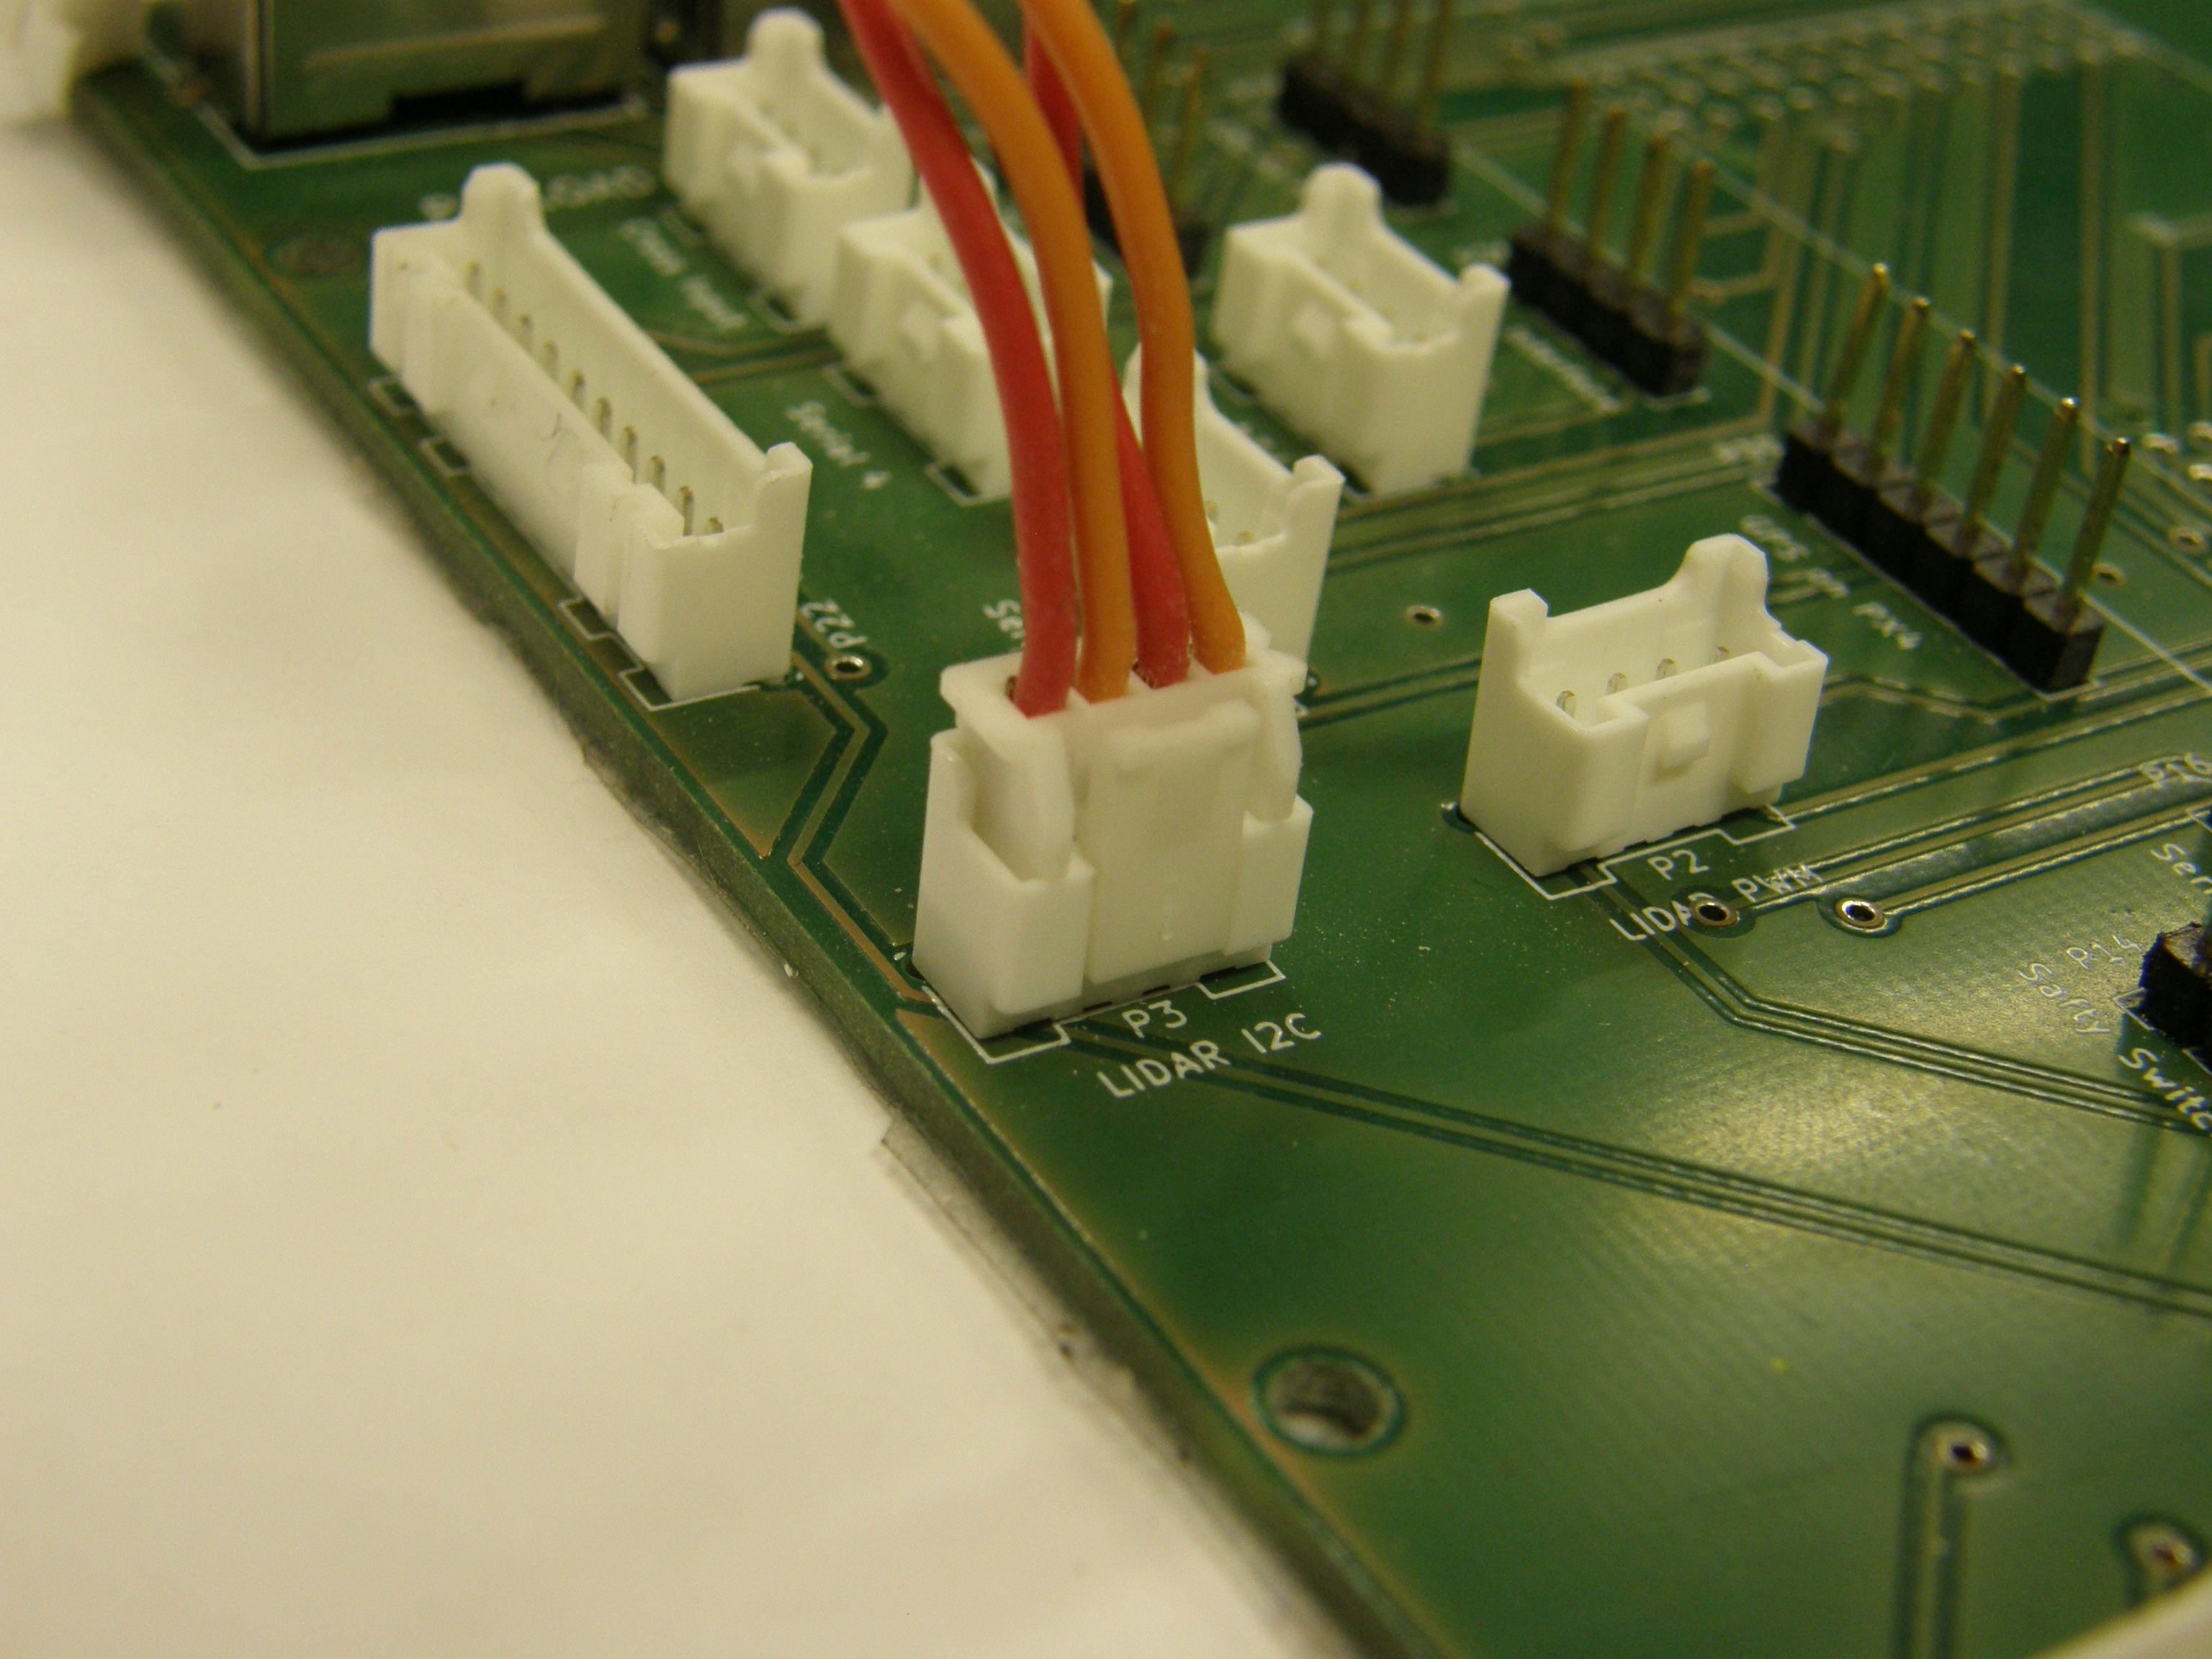
\includegraphics[width=0.6\textwidth, center]{bilder/Stecker/Stecker_JST_PA.jpg} 
\caption{Der mittlerweile eingesetzte JST PA Steckverbinder} 
\label{fig:Der mittlerweile eingesetzte JST PA Steckverbinder}
\end{subfigure}

\end{figure}

Generell soll weiter ein Standardisierung der Verbinder erfolgen und Vollständig eine Fixierung durch Formschluss etabliert werden.
Als Hemnis bei der Erprobung neuer Verbinder muss generell aber auch die Verarbeitungsinvestitionen bedacht werden. Zwar sind die Stecker und Buchsen als Bauteile Günstig in der Anschaffung. Jedoch kosten Crimpwerkzeuge in Vertretbarer Qualität ohne weiteres mehrere Hundert Euro für jedes neue Steckersystem.





\subsection{Priorisierung externer Anschlüsse im Ground Handling}

Die Priorisierung bestimmter Energiequellen wurde erstmals in der Saison 2016 eingesetzt.
Damit wurde es möglich, an einen Flugfertig Montierten System alle Vorflugkontrollen und die Kalibrierung der Autopilotensysteme durchzuführen ohne die Missionsenergieversorgung zu entladen. Dazu wurde ein ähnlicher Akku mit ebenfalls vier Zellen an einem Zentralen Anschluss in der sogenannten WingCenterBox Verbunden. Solange dieser Angeschlossen war wurde sämtliche Energie für die Steuerelektronik, die Servosysteme und die Motortesläufe ausschließlich aus diesem bezogen. Die zentrale Unterbringung des Anschlusspunktes in der WingCenterBox stellte sicher das ein Schließen der CenterBox Abdeckung nur nach vorheriger Demontage des externen Akkus möglich war, was Bedienungsfehler ausschloss.

\begin{figure}[H]
\centering
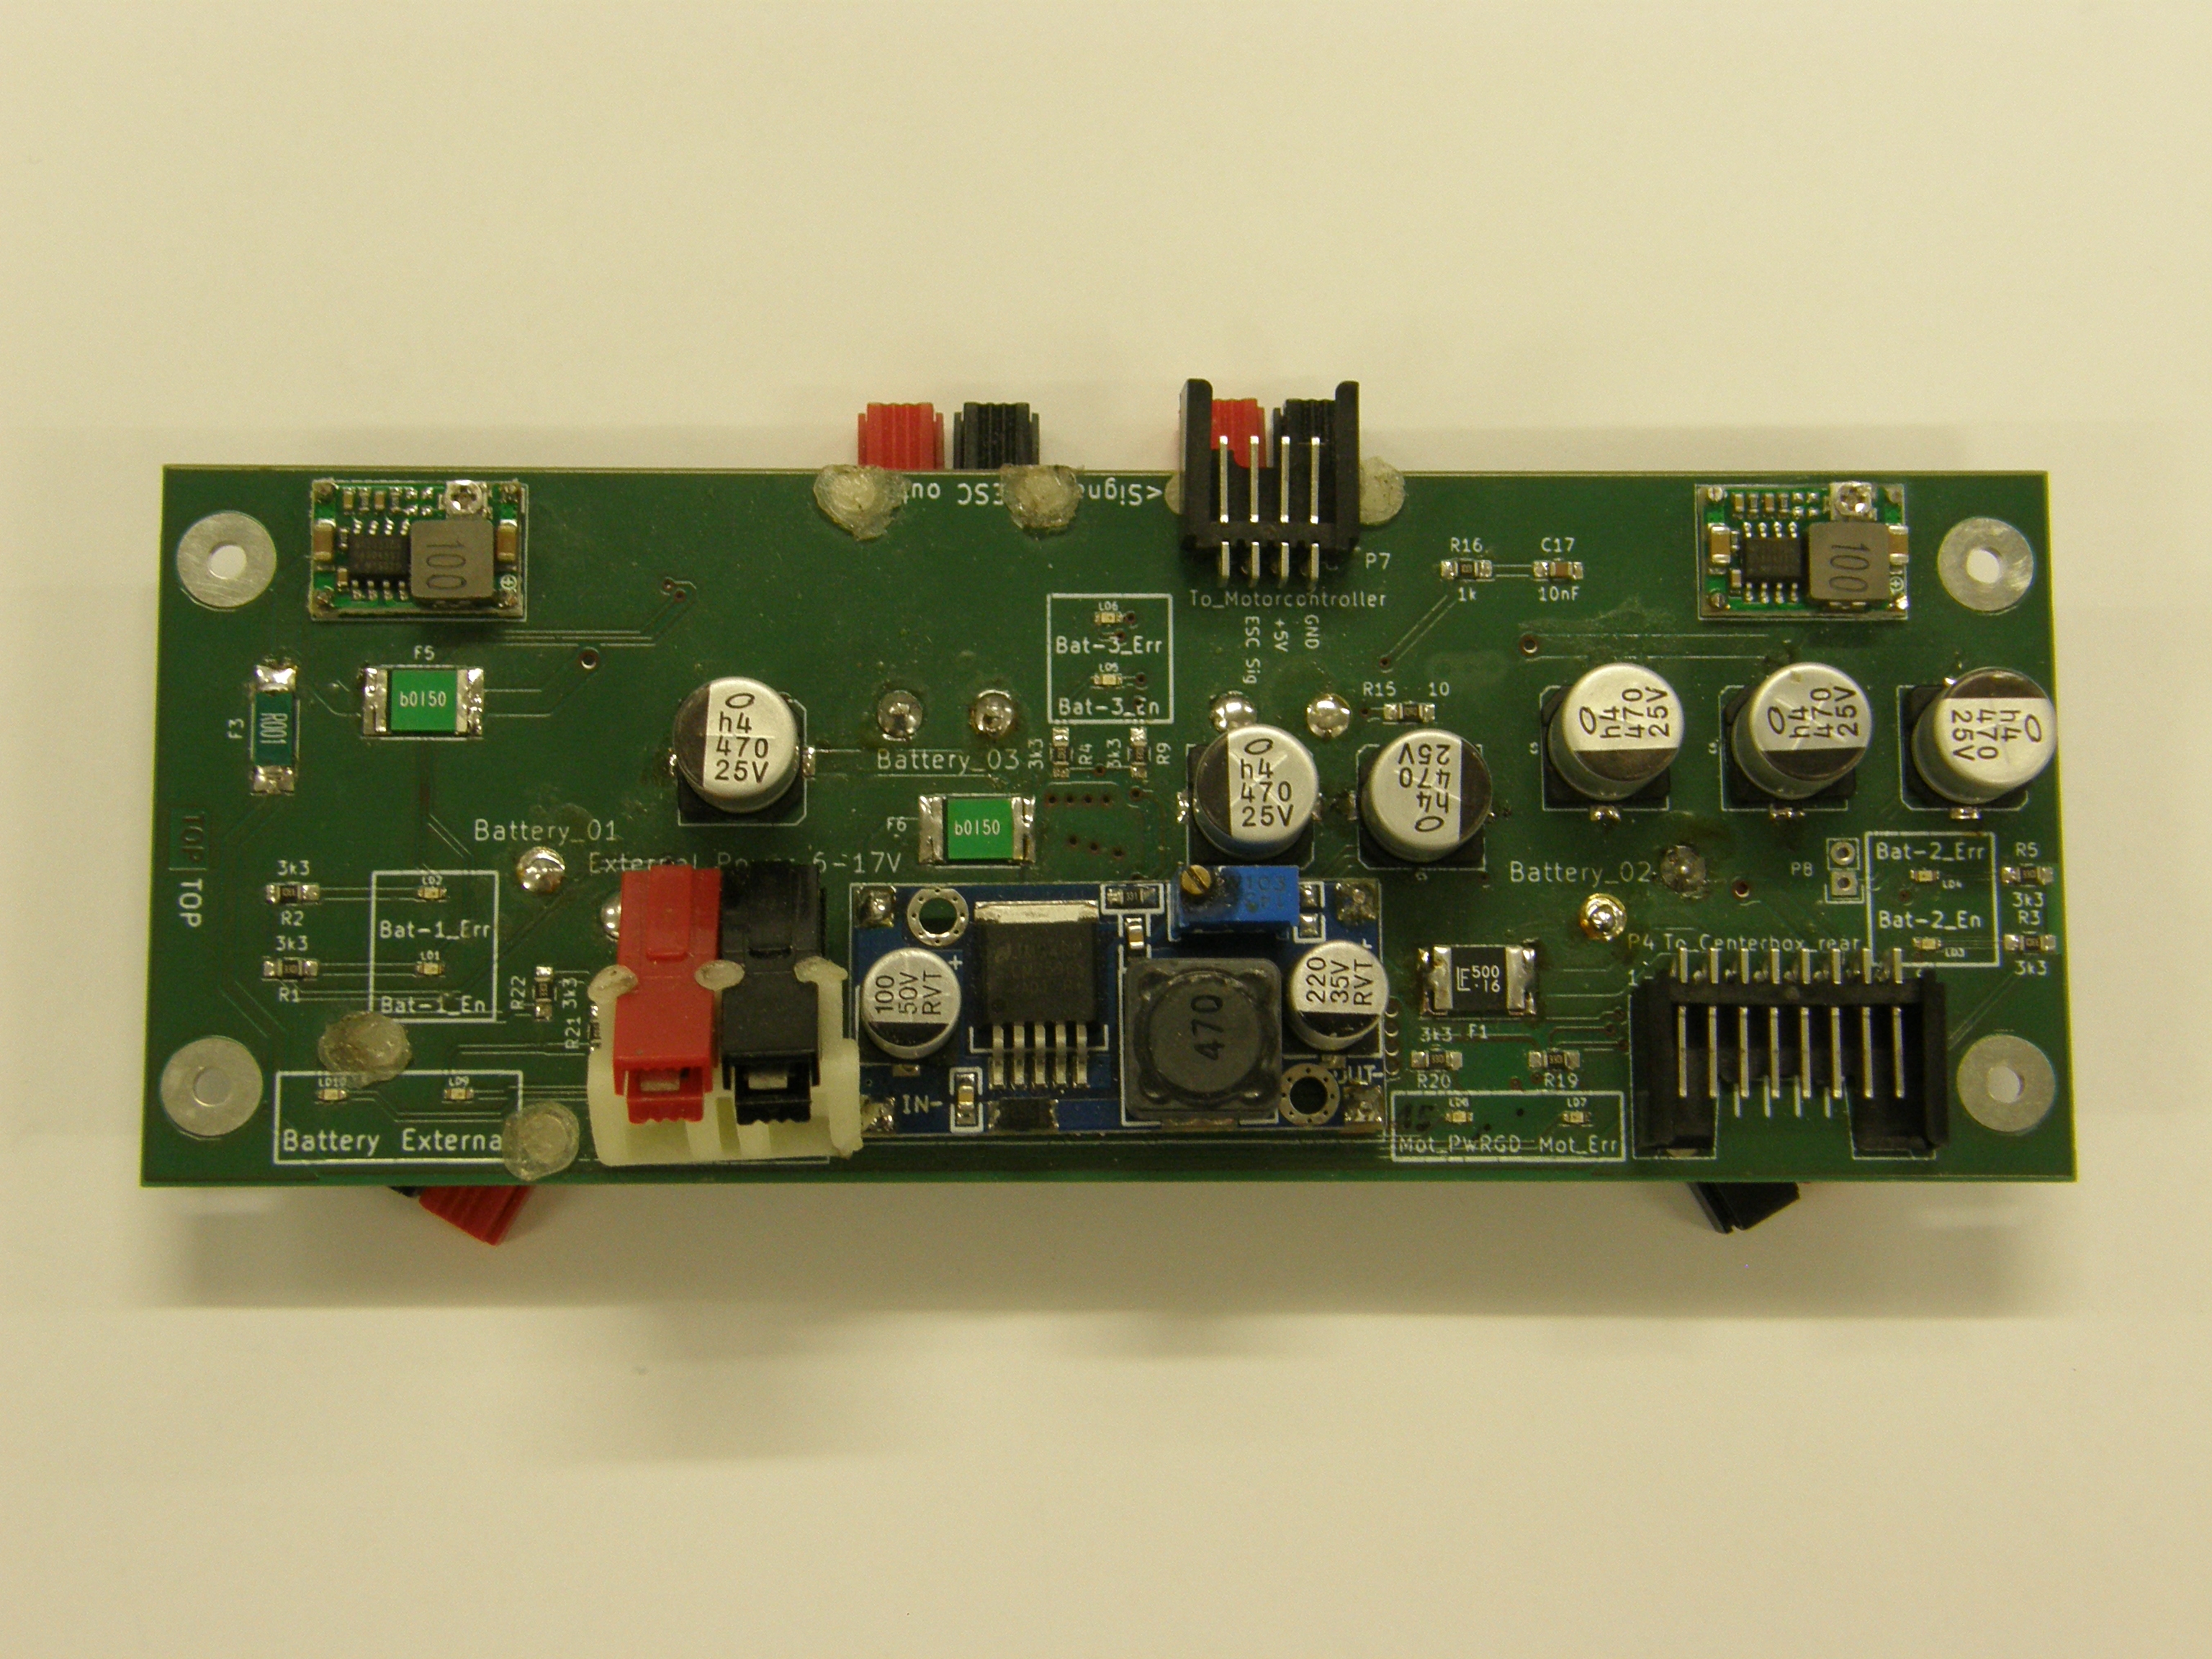
\includegraphics[width=0.9\textwidth]{bilder/Centerbox/Centerbox-Front_Power_AUVSI_2016_Oberseite.jpg} 
\caption{Blick auf die Externen Anschlüsse der AUVSI 2016 Platine} 
\label{fig:Blick auf die Externen Anschlüsse der AUVSI 2016 Platine}
\end{figure}

-->>Schaltplan 2016 


\subsection{Schutz vor Fehlbedienung im Leistungspfad}

Da Fehler abseits von Verbindungsproblemen im Leistungspfad quasi immer zur Beschädigung oder zur Zerstörung des selbigen, mit potentiellem Personenschaden führen, werden für diesen die meisten Sicherheitsmechanismen verwendet.
Hauptsächlich wird das Ideale Dioden System verwendet um einen parallelen Betrieb von Akkus verschiedener Ladungsstände zu ermöglichen.

\subsubsection{Die Ideale Diode}

Die Ideale Diode als Elektronische Schaltung lässt sich in ihrem Schematischen Aufbau mit folgendem Schaltplan darstellen.

\begin{figure}[H]
\centering
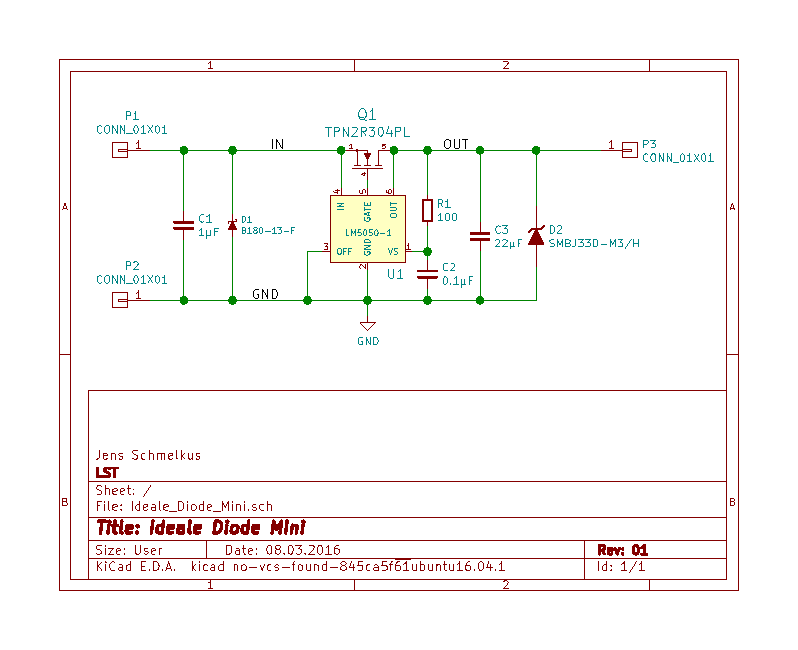
\includegraphics[width=0.9\textwidth]{Schaltplaene/Ideale_Diode_Mini.pdf} 
\caption{Schaltplan der Idealen Diode erster Generation} 
\label{fig:Schaltplan der Idealen Diode erster Generation}
\end{figure}

Grundlegend Besteht der Aufbau aus einem Steuermodul und einem Schalter. Außerdem werden ein und Ausgänge der Aufbaus mit Spannungsdämpfern und Verpolungs- sowie Überspannungsschutz versehen.



\subsubsection{Die Ideale Diode als Modul}

Um eine leichte Integration in möglichst viele Anwendungen zu ermöglichen wurde beim Layout der Platine die kleinstmögliche Abmessung angestrebt. 

\begin{figure}[H]
\centering
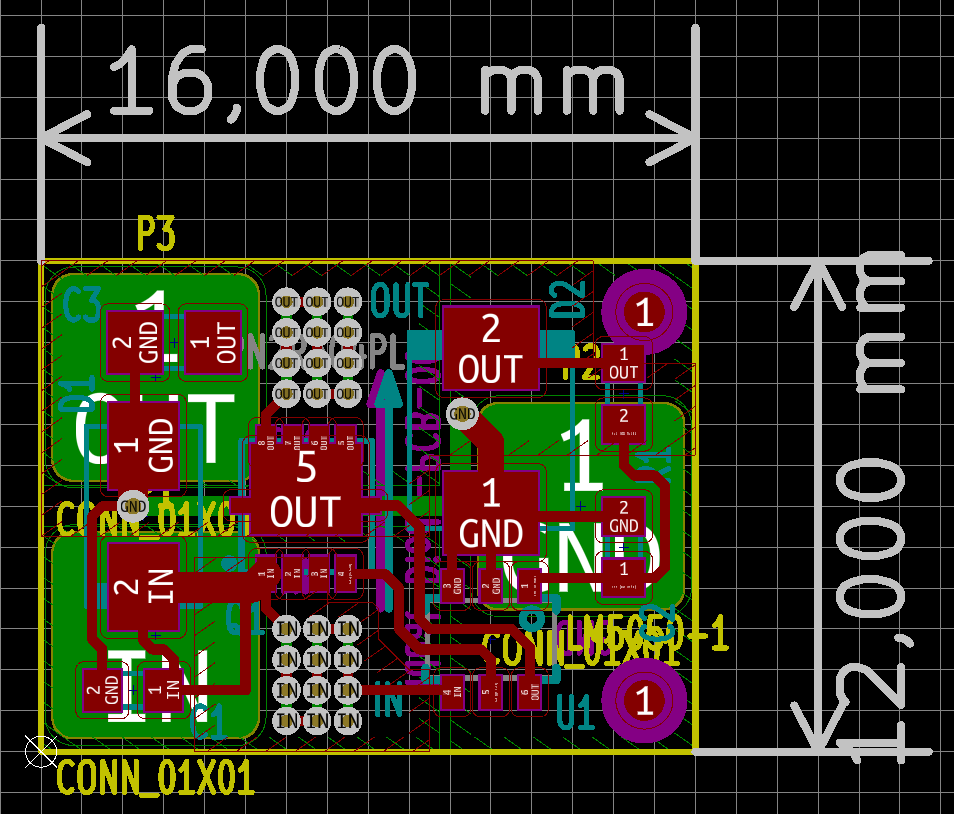
\includegraphics[width=0.9\textwidth]{bilder/Ideale_Diode/Ideale_Diode_Mini_rev01_ver00.png} 
\caption{Layout der Idealen Diode erster Generation} 
\label{fig:Layout der Idealen Diode erster Generation}
\end{figure}

Damit ergab sich in der Montage ein kompaktes Baumaß für die Platine mit all ihren Bauelementen.

\begin{figure}[H]
\centering
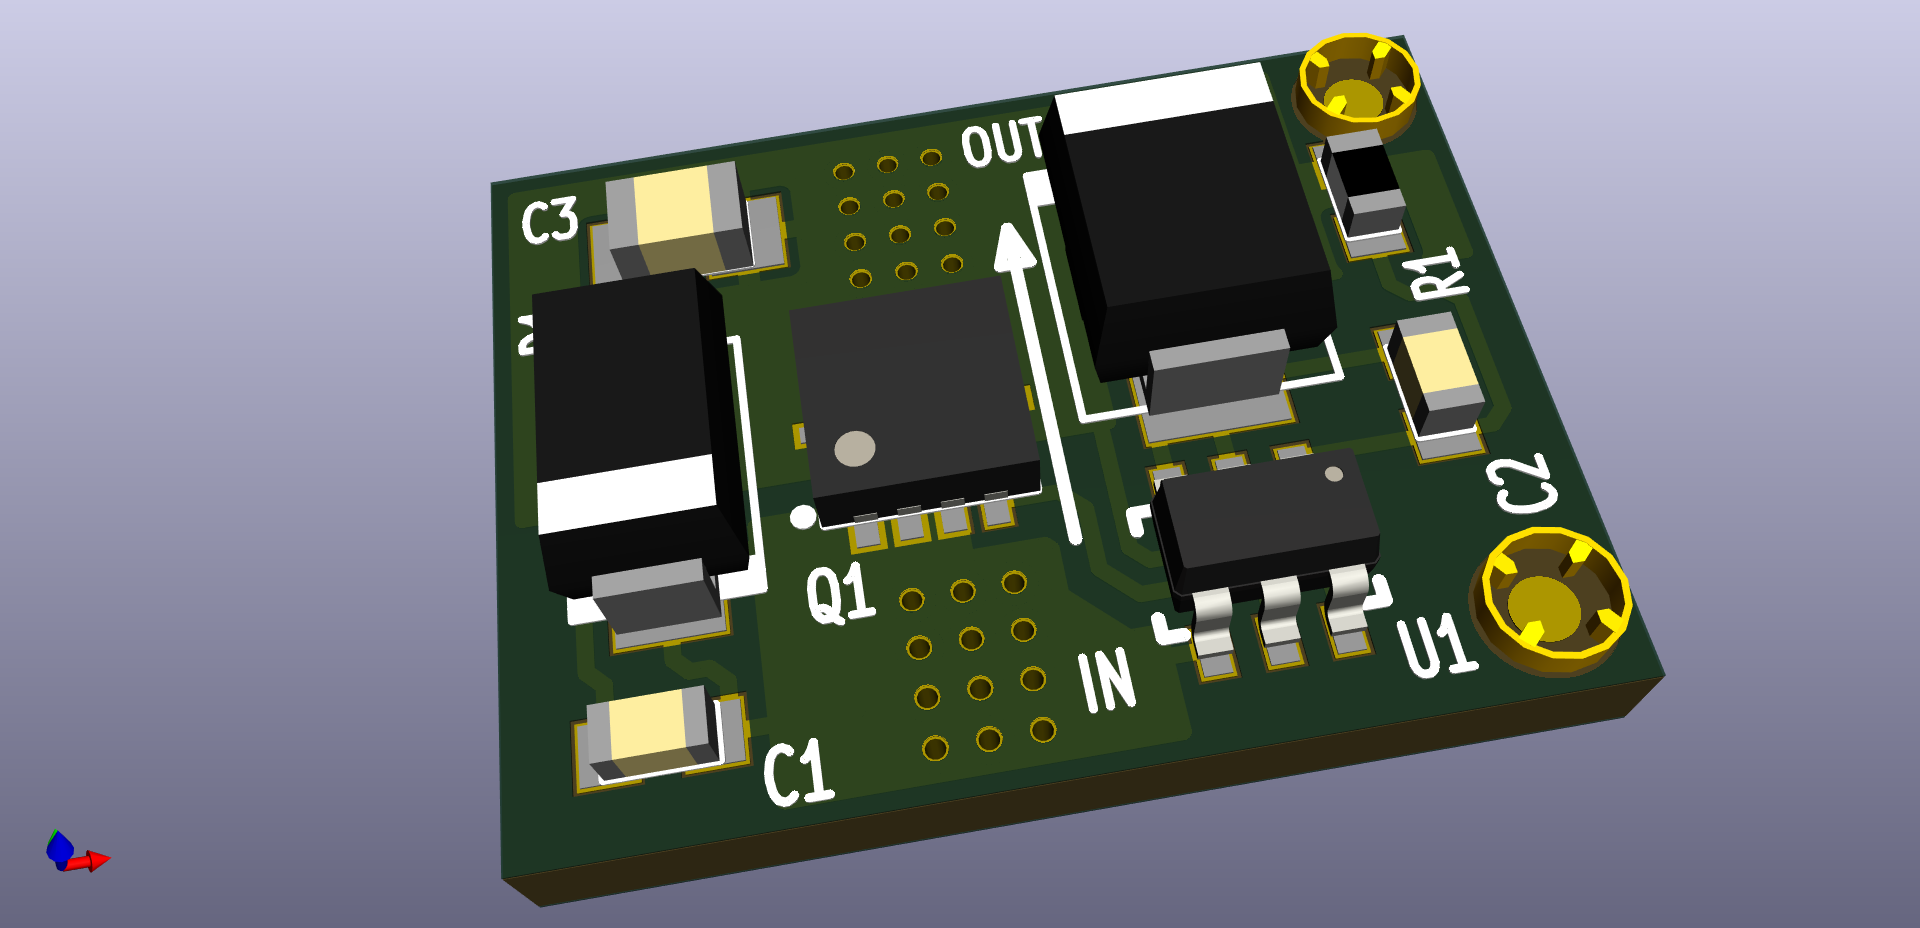
\includegraphics[width=0.9\textwidth]{bilder/Ideale_Diode/Ideale_Diode_Mini_rev01_ver00-3D.png} 
\caption{3D Ansicht der Idealen Diode erster Generation} 
\label{fig:3D Ansicht der Idealen Diode erster Generation}
\end{figure}

\subsubsection{Optimierung der Idealen Diode}

Nach den Messungen zur Verlustleistung an der idealen Diode wurde die Abhängigkeit von Kühlung und Innenwiderstand des Mosfets quantifiziert. 


\begin{figure}[H]
\centering
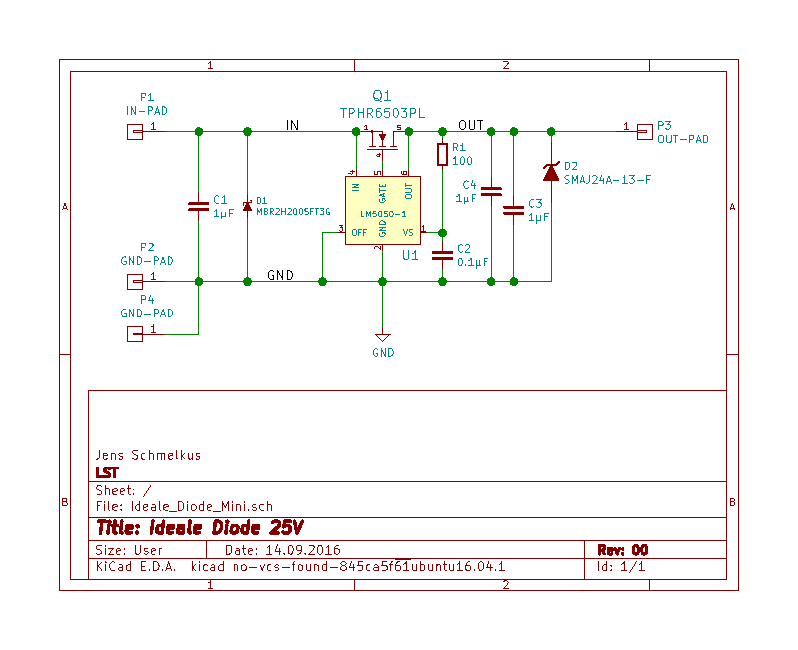
\includegraphics[width=0.9\textwidth]{Schaltplaene/Ideale_Diode_25V_rev00-ver00.pdf} 
\caption{Schaltplan der Idealen Diode zweiter Generation} 
\label{fig:Schaltplan der Idealen Diode zweiter Generation}
\end{figure}


\begin{figure}[H]
\centering
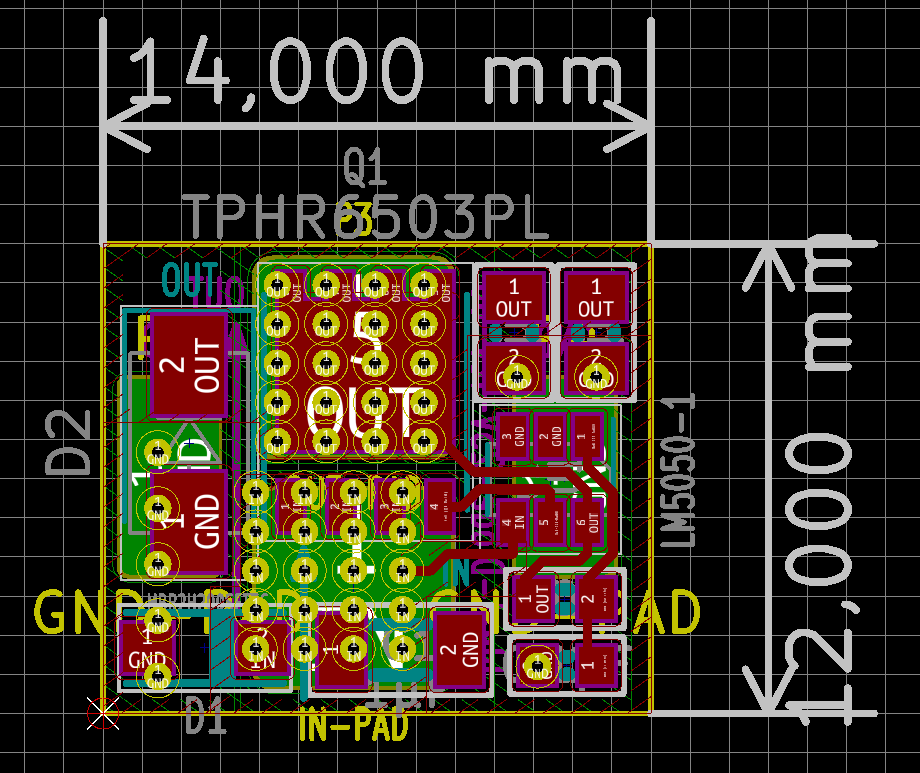
\includegraphics[width=0.9\textwidth]{bilder/Ideale_Diode/Ideale_Diode_25V_rev00_ver00.png} 
\caption{Layout der Idealen Diode zweiter Generation} 
\label{fig:Layout der Idealen Diode zweiter Generation}
\end{figure}



\begin{figure}[H]
\centering
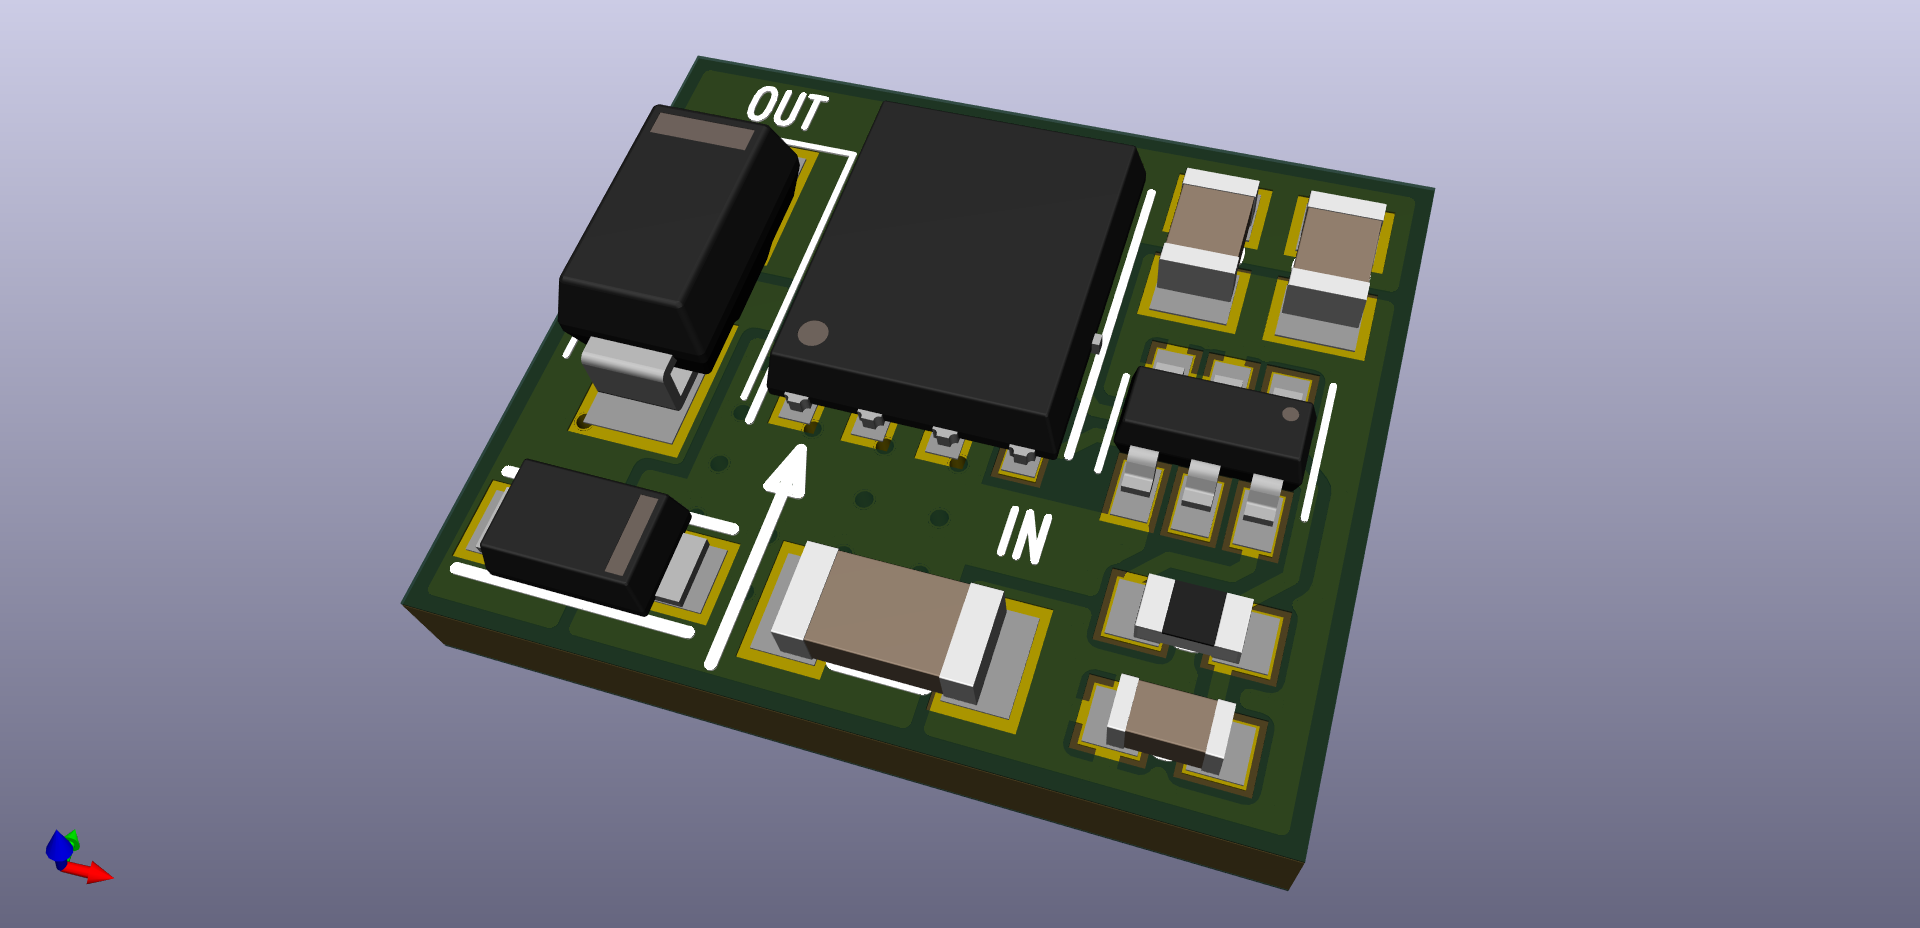
\includegraphics[width=0.9\textwidth]{bilder/Ideale_Diode/Ideale_Diode_25V_rev00_ver00-3D.png} 
\caption{3D Ansicht der Idealen Diode zweiter Generation} 
\label{fig:3D Ansicht der Idealen Diode zweiter Generation}
\end{figure}


\begin{figure}[H]
\centering
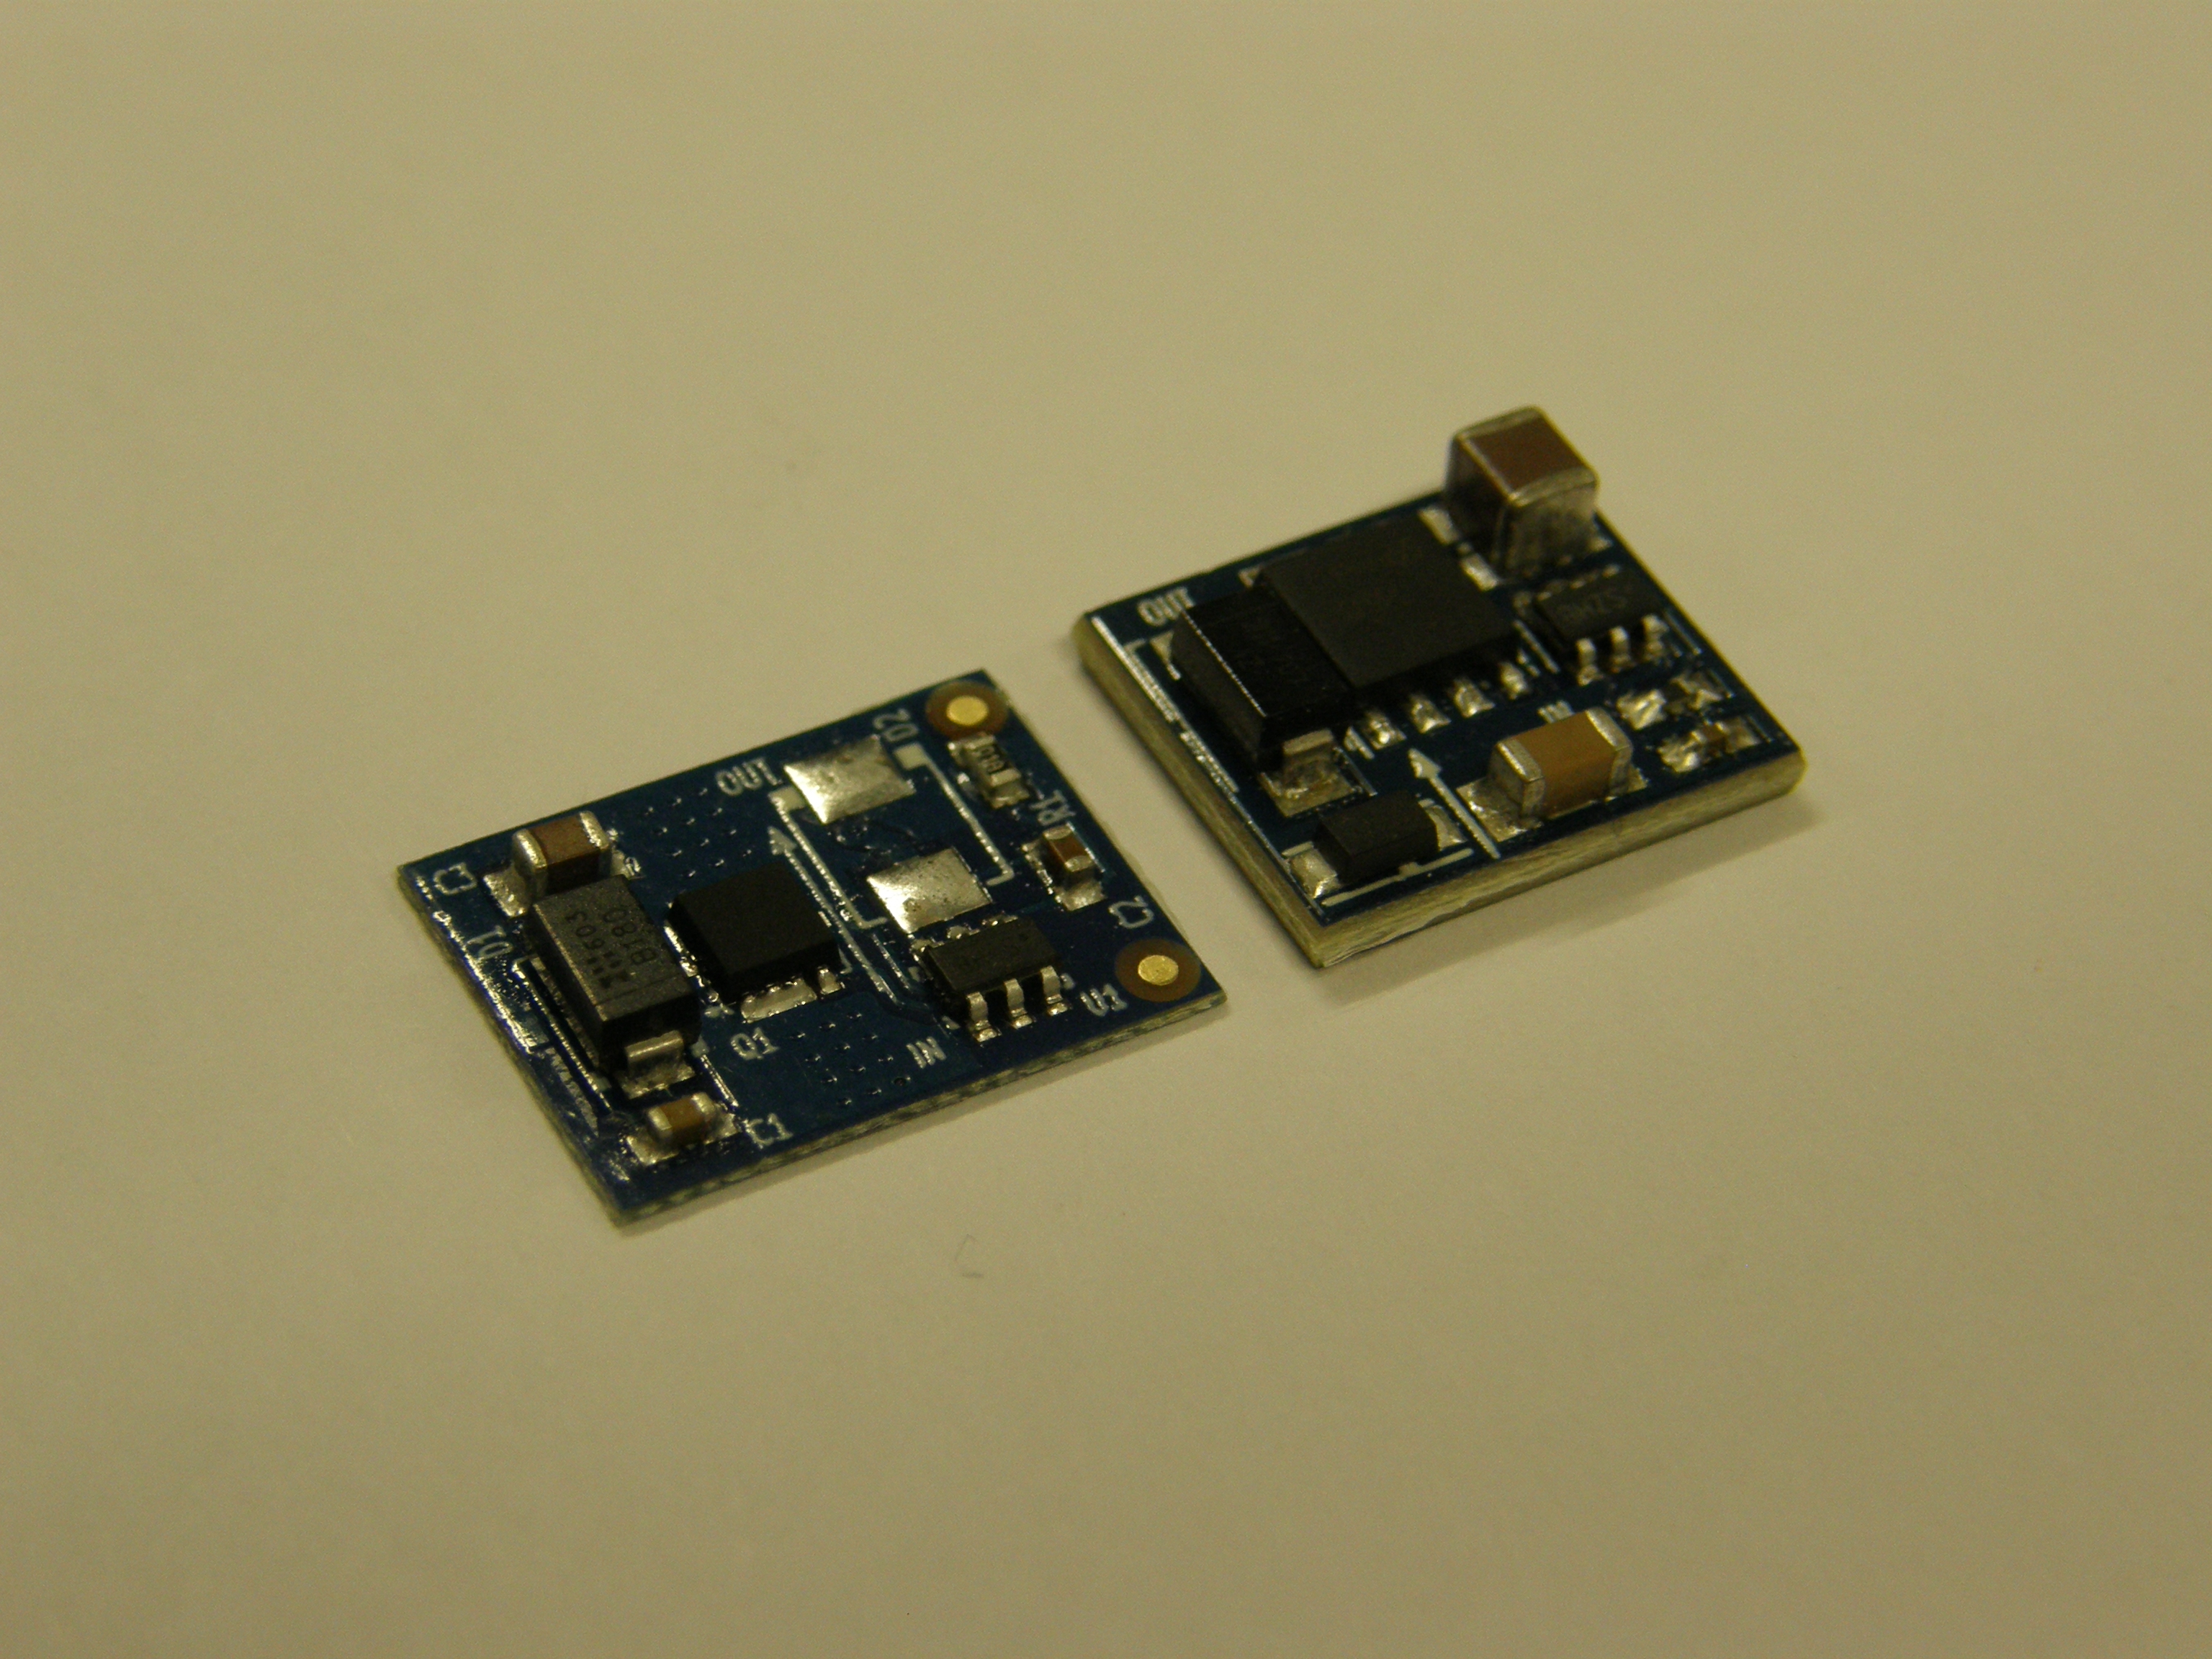
\includegraphics[width=0.9\textwidth]{bilder/Ideale_Diode/Ideale_Dioden_Paar_dreiviertel.jpg} 
\caption{Beide Generationen des Ideale Dioden Moduls nebeneinander} 
\label{fig:Beide Generationen des Ideale Dioden Moduls nebeneinander}
\end{figure}

\section{Integration von Zukaufbaugruppen}


LM2596S  Baugruppe Dc-Dc 
Vin 4 - 35 V 

Vout 1,23 - 30 V einstellbar

3 A  mit Kühlung

meist auf 5V  eingestellt 
Meist 5V Versorgung für Servos

\begin{figure}[H]
\centering
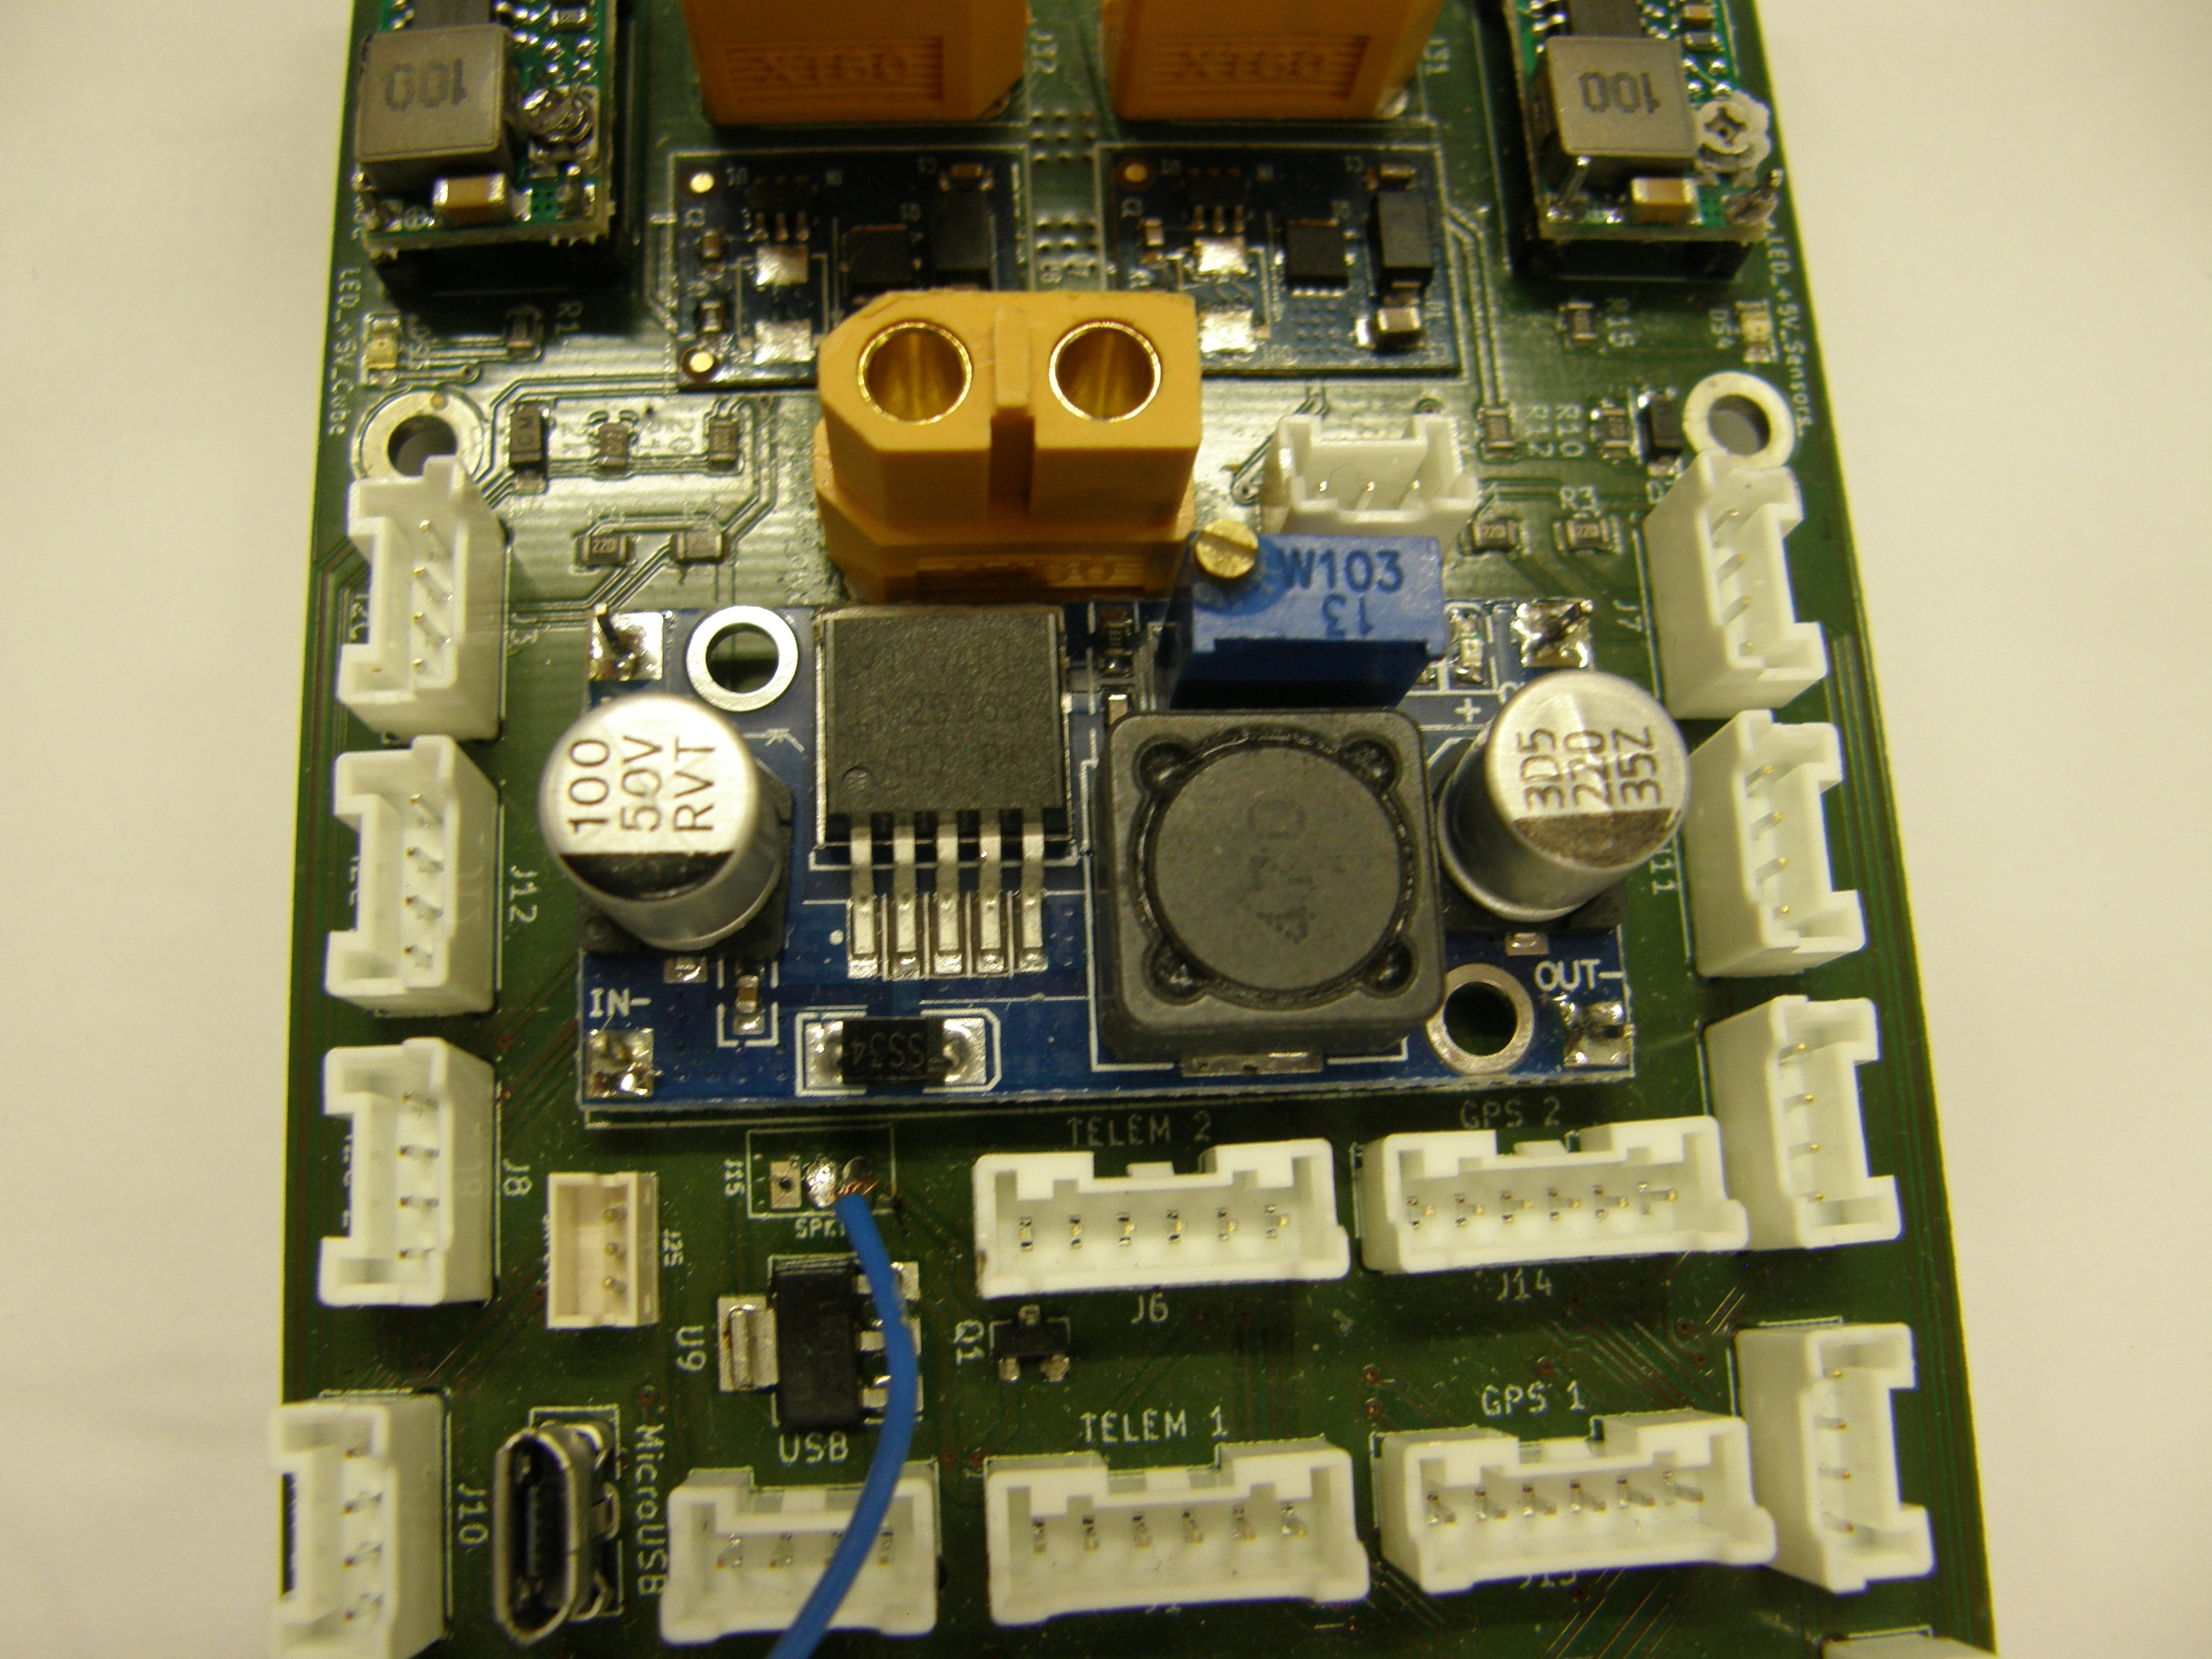
\includegraphics[width=0.9\textwidth]{bilder/Zukaufbauteile/Baugruppen_Dc-Dc_LM2596S.jpg} 
\caption{Zugekauftes Dc-Dc Wandler PCB mit LM2596} 
\label{fig:Zugekauftes Dc-Dc Wandler PCB mit LM2596}
\end{figure}


DSN Mini 360  Baugruppe Dc-Dc

Vin 4,75 - 23 V

Vout 1,0 - 17 V einstellbar

Iout dauer  ~ 1,5 A

Meist 5 V versorgung für Pixhawk und Lidar

\begin{figure}[H]
\centering
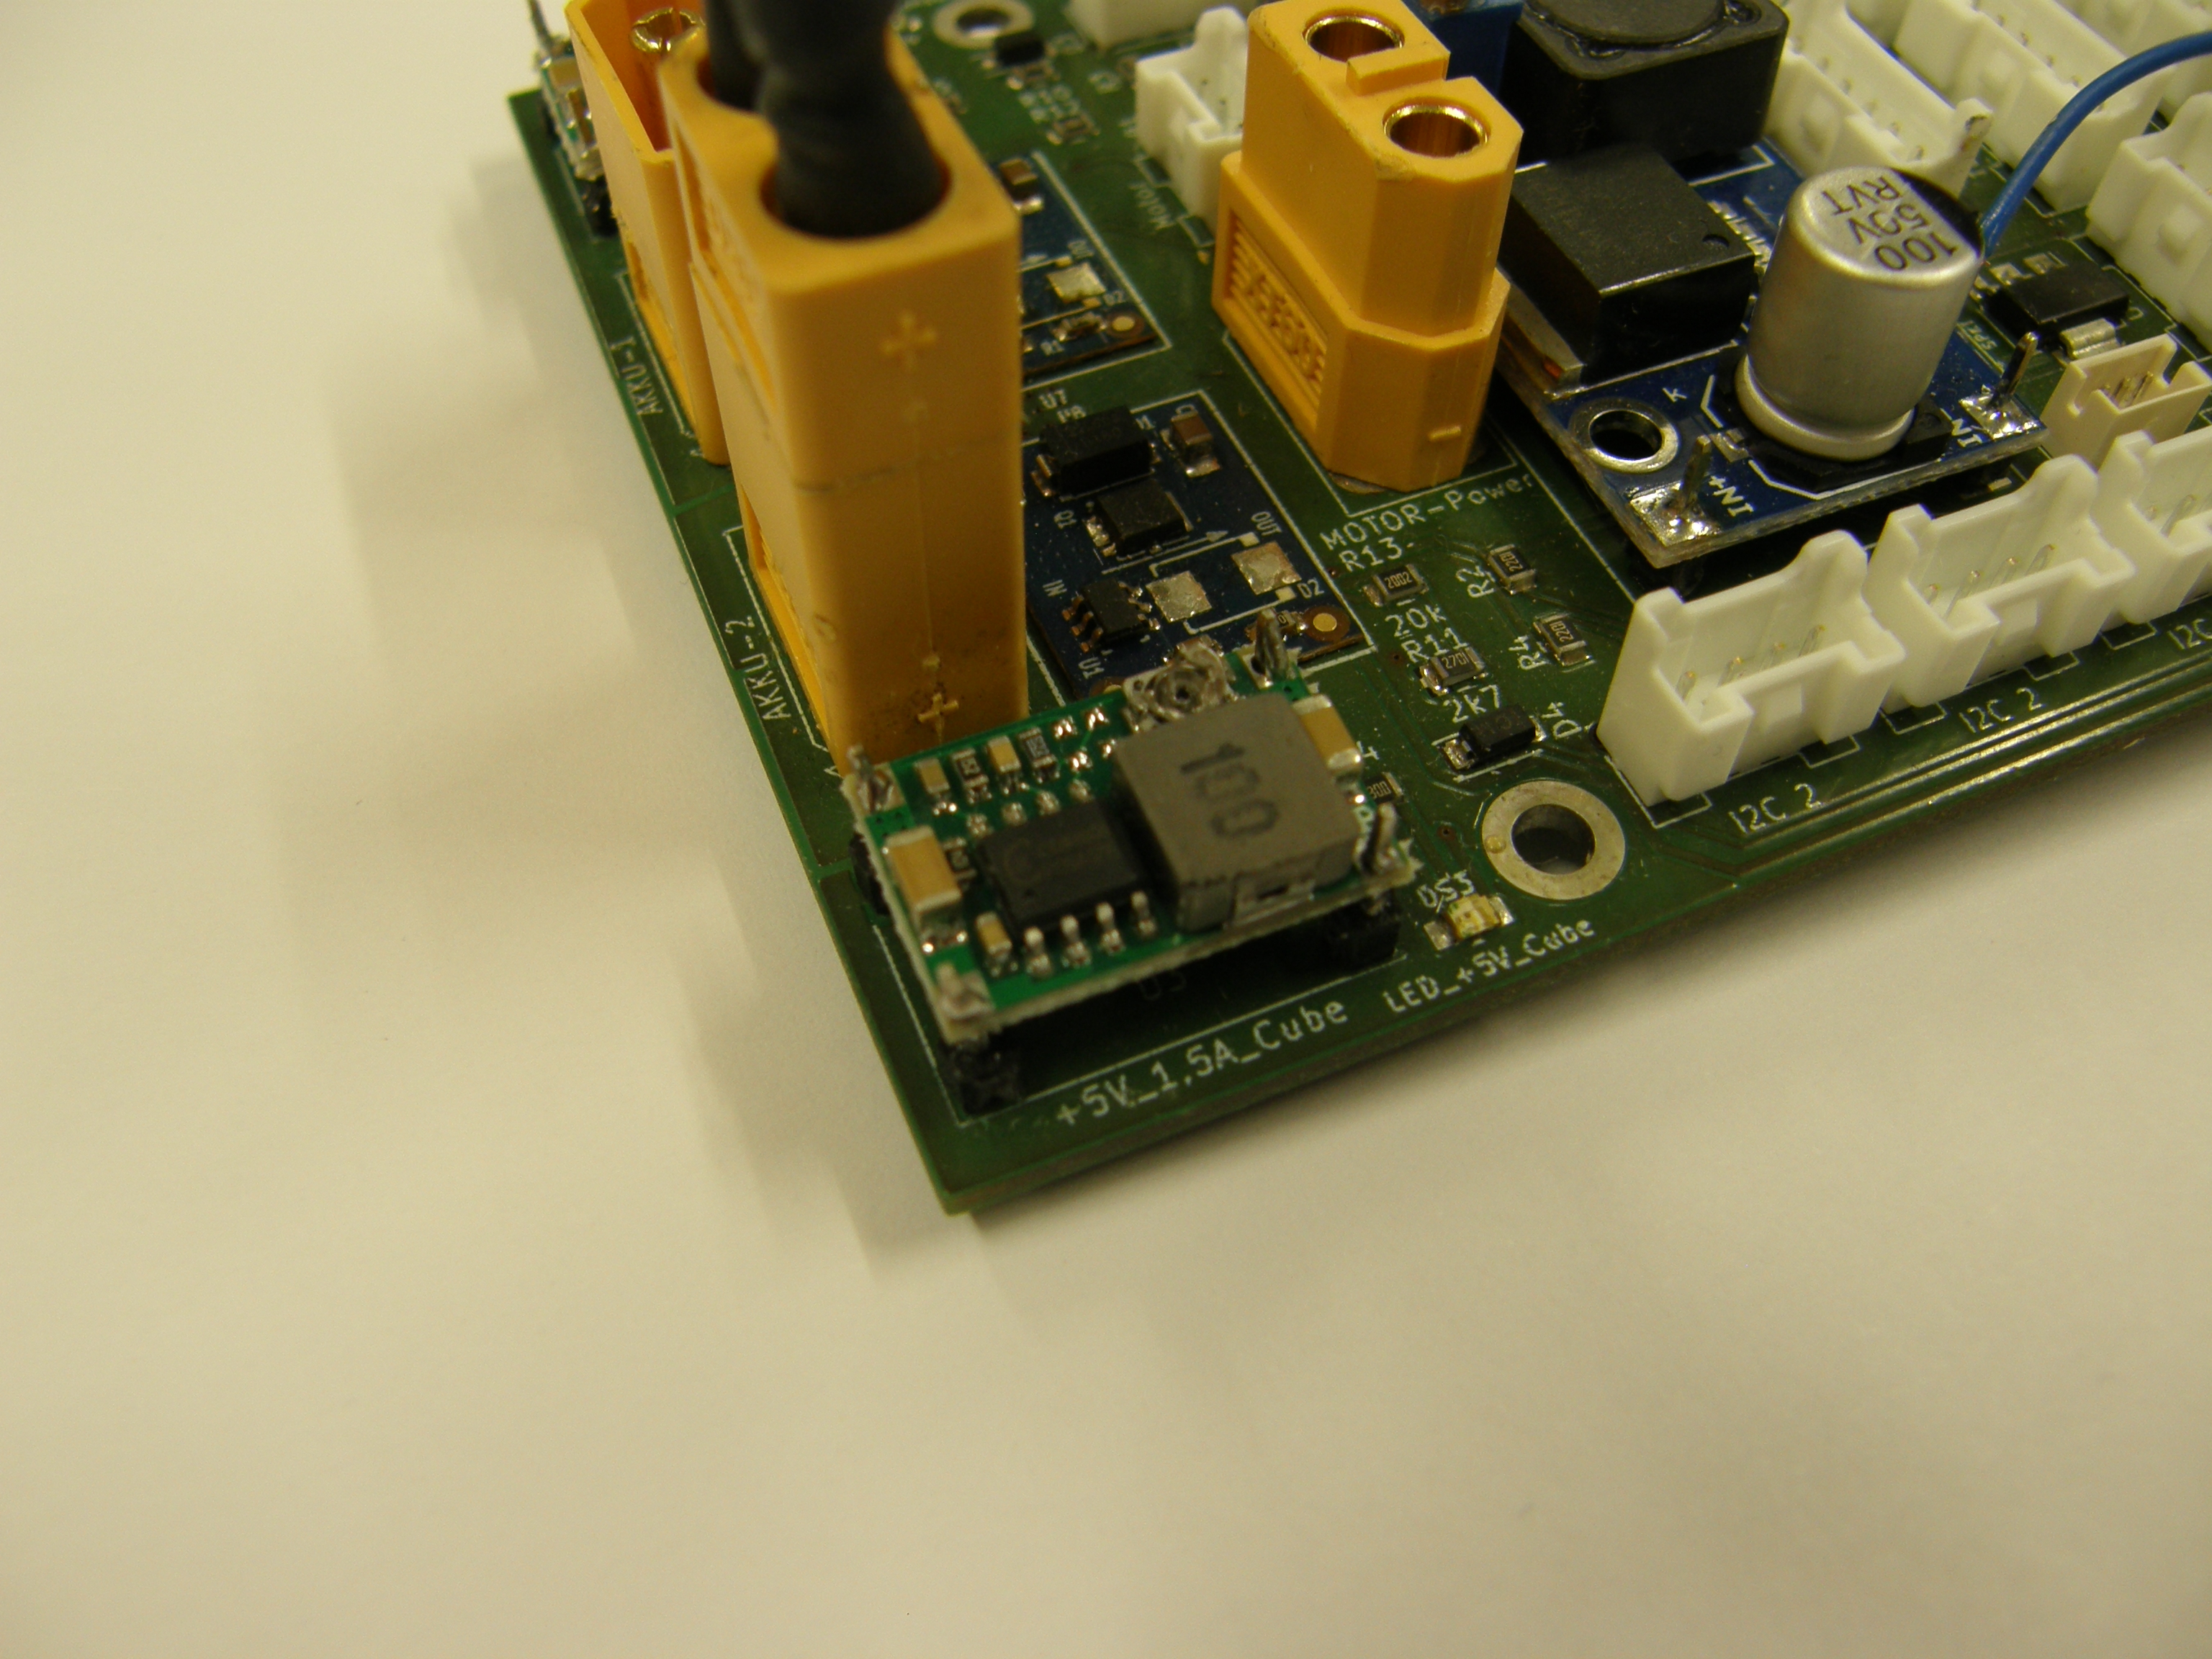
\includegraphics[width=0.9\textwidth]{bilder/Zukaufbauteile/Baugruppen_Dc-Dc_Mini-360.jpg} 
\caption{Zugekauftes Dc-Dc Wandler PCB Mini-360} 
\label{fig:Zugekauftes Dc-Dc Wandler PCB Mini-360}
\end{figure}

\section{Mechanische Integration im Flugsystem}

\begin{figure}[H]
\centering
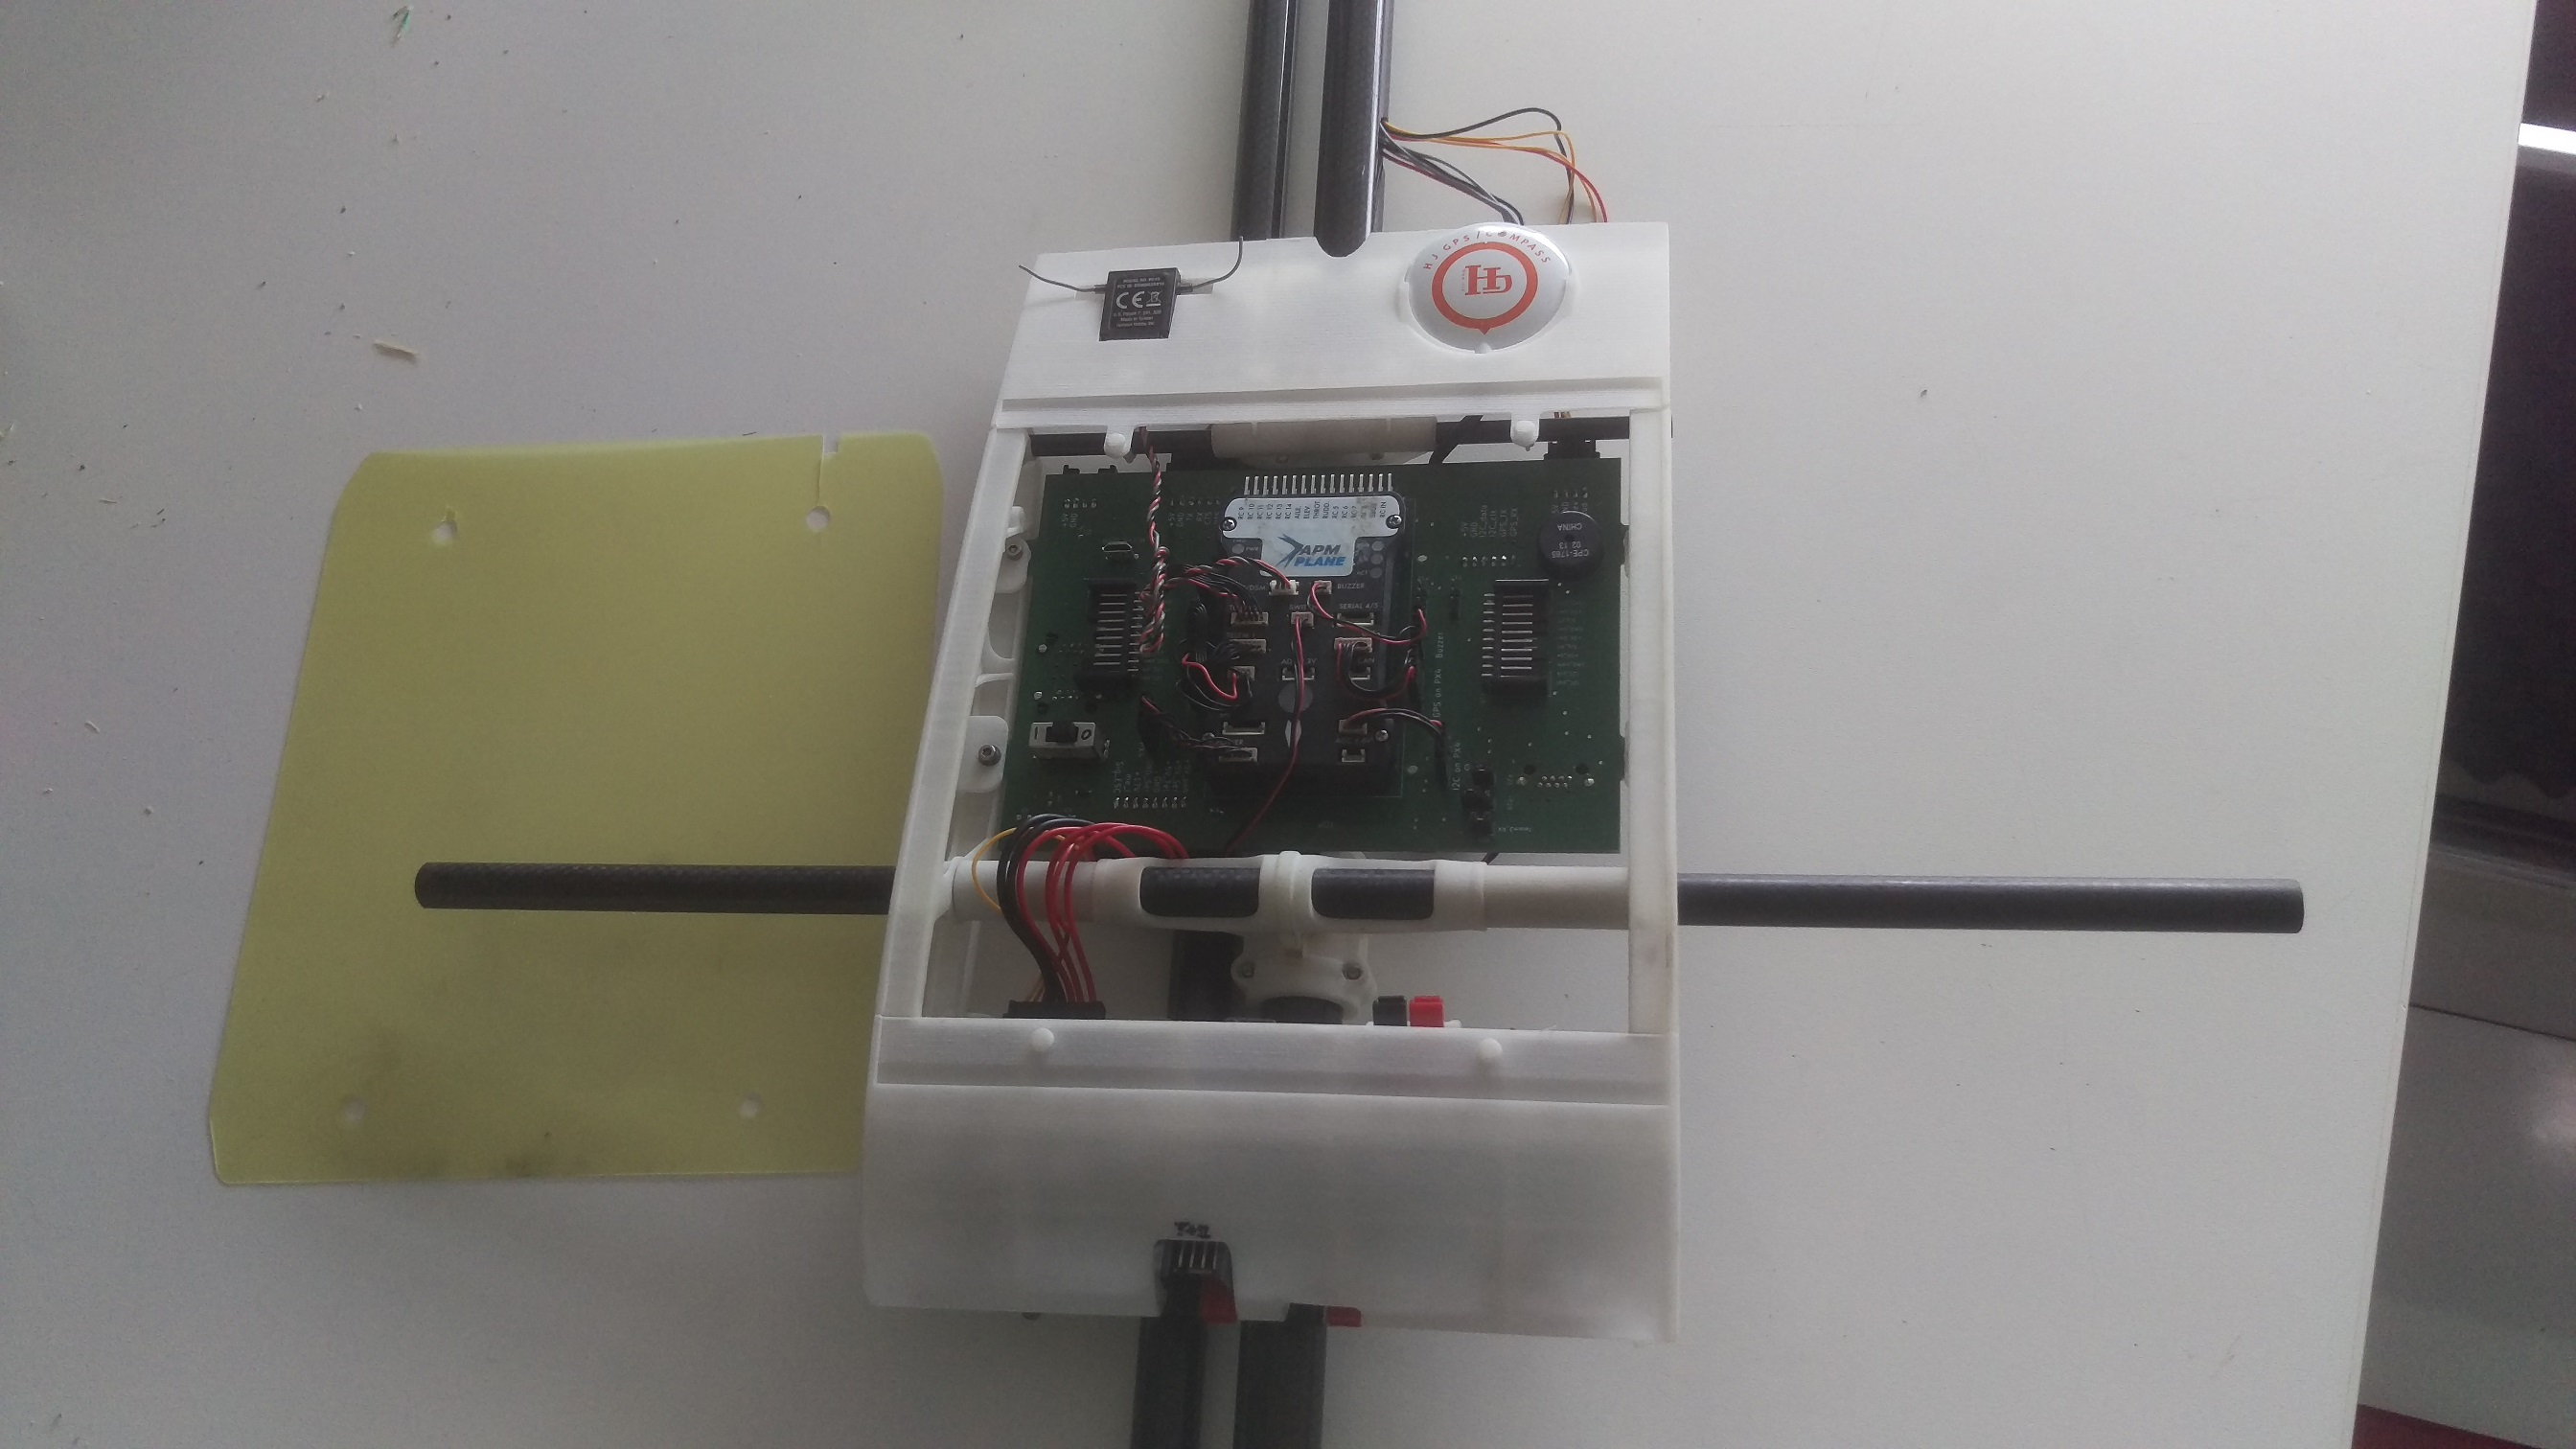
\includegraphics[width=0.9\textwidth]{bilder/Fotos/AUVSI_2016_Centerbox_Detail.jpg} 
\caption{In der WingCenterBox eingebaute Autopilotenplatine} 
\label{fig:In der WingCenterBox eingebaute Autopilotenplatine}
\end{figure}